\chapter{Le détecteur Compact Muon Solenoid (CMS)}
\renewcommand\chapterillustration{CMS/cms.jpeg}
\ThisULCornerWallPaper{1}{\chapterillustration}
\minitoc

\section{Le détecteur Solénoïde compact à muons (CMS)}
Le détecteur Solénoïde compact à muons abrégé en CMS (pour Compact Muon Solenoid) est avec ATLAS une expérience généraliste qui a comme buts majeurs :

\begin{itemize}[label=$\bullet$]
	\item \textbf{La recherche du boson de Higgs : } Lors de la conception de CMS dans les années 1990, la détection du boson de Higgs à été prise comme référence afin de tester les performances du design du détecteur. Ce but à été réalisé avec la découverte d'une particule compatible avec le boson de Higgs le 4 juillet 2012 (cf.\ref{higgs}).
	\begin{figure}[h!]
		\subfloat[Distribution de la masse invariante en mode diphoton, chaque événement étatnt pondéré par S/(s+b) les traits représente le signal et le bruit de fond. Les bandes rpersente les incertitudes décart type $\pm$1 et $\pm 2$ dans l'estimation du bruit de fond.L'encart montre la partie centrale de la distribution de masse invariante non pondérée]{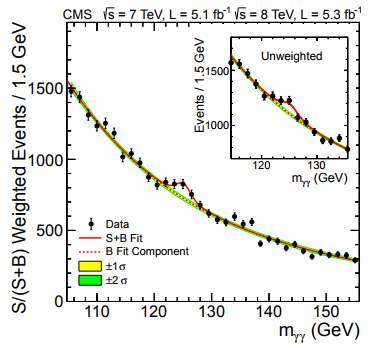
\includegraphics[width=.48\linewidth]{CMS/higgs1.png}}
		\subfloat[Distribution de la masse invariante pour $ZZ\rightarrow 4l$/ Les points représentent les données, l'histogramme plein le bruit de fond et l'histogramme creux le signal pour un boson de Higgs de mass $m_{h}=125$ GeV ajouté au bruit de fond/]{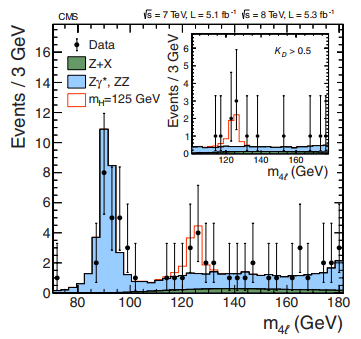
\includegraphics[width=.48\linewidth]{CMS/higgs2.png}}
		\caption{Deux de la masse invariante dans des canaux de désintégration du boson de Higgs montrant sa découverte.[paper]}
		\label{higgs}
	\end{figure}
	\item \textbf{Confirmer et préciser les mesures de la physique du Modèle Standard : } Des mesures de précisions dans des domaines tels que la QCD, le couplage électrofaible, et la physique des saveurs pourrait donner des indications d'une physique au-dlà du Modèle Standard.
	\item \textbf{La recherche de signes de physique au-delà du Modèle Standard : }CMS permet la recherche de particules supersymmétriques ou de nouveaux bosons vecteur massifs ($Z'$) ou encore la recherche de dimensions supplémentaires par exemple.
	\item \textbf{Étudier les collisions d'ions lourds.}
\end{itemize}

Afin de répondre à ses objectifs, le "Technical Design Report" (TDR) a fixé le cahier des charges et les caractéristiques essentielles du détecteur CMS, à savoir :
\begin{itemize}[label=$\bullet$]
	\item Une bonne identification des muons et une bonne résolution en impulssion sur une vaste gamme d'impulssion pour la région $|\eta|<2.5$, une bonne résolution en masse pour les dimuons ($\approx 1\%$ à 100GeV/c$^{2}$) et la capacité à déterminé de manière certaine la charge des muons de $p<$ 1TeV/c.
	\item Une bonne résolution en impulssion pour les particules chargées ainsi qu'une bonne efficacuté de reconstruction dans le trajectographe interne (inner tracker). Un déclenchement et un étiquettage efficace pour les jets venant de quarks $\tau$ et $b$, ce qui requiert un détecteur à pixels proche du point d'interaction.
	\item Une bonne résolution pour l'énergie électromgnétique, et une bonne résolution en masse pour les diphoton et dielectron  ($\approx 1\%$ à 100GeV/c$^{2}$), une grande couverture géométrique ($|\eta|<2.5$), une mesure de la diraction des photons et/ou une correction localisation du vertex primaire d'interaction ainsi qu'une bonne rejection des $\pi_{0}$ et une isolation des photons et letptons efficace à haute luminosité.
	\item une bonne résolution en masse des dijets et une bonne résolution en masse de l'énergie transverse manquante $E_{T}^{miss}$. Ceci requiert un calorimètre hadronique hermétique de très grande couverture géométrique ($|\eta|<5$) et une fine segmentation latérale ($\Delta\nu\times\Delta\Psi<0.1\times0.1$)
\end{itemize} 

\subsection{Description générale de CMS}
Le détécteur CMS se trouve dans une caverne situé au point 5 (P5), proche du village de Cessy en France. La construction de CMS s'est effectué en surface et par tranches autonomes afin de réduire le temps et les coûts nécessaire à sa construction. Chaque tranche à ensuite été descendu dans la caverne et assemblé à 100 m sous terre (cf.fig\ref{slice}).
\marginpar
{
	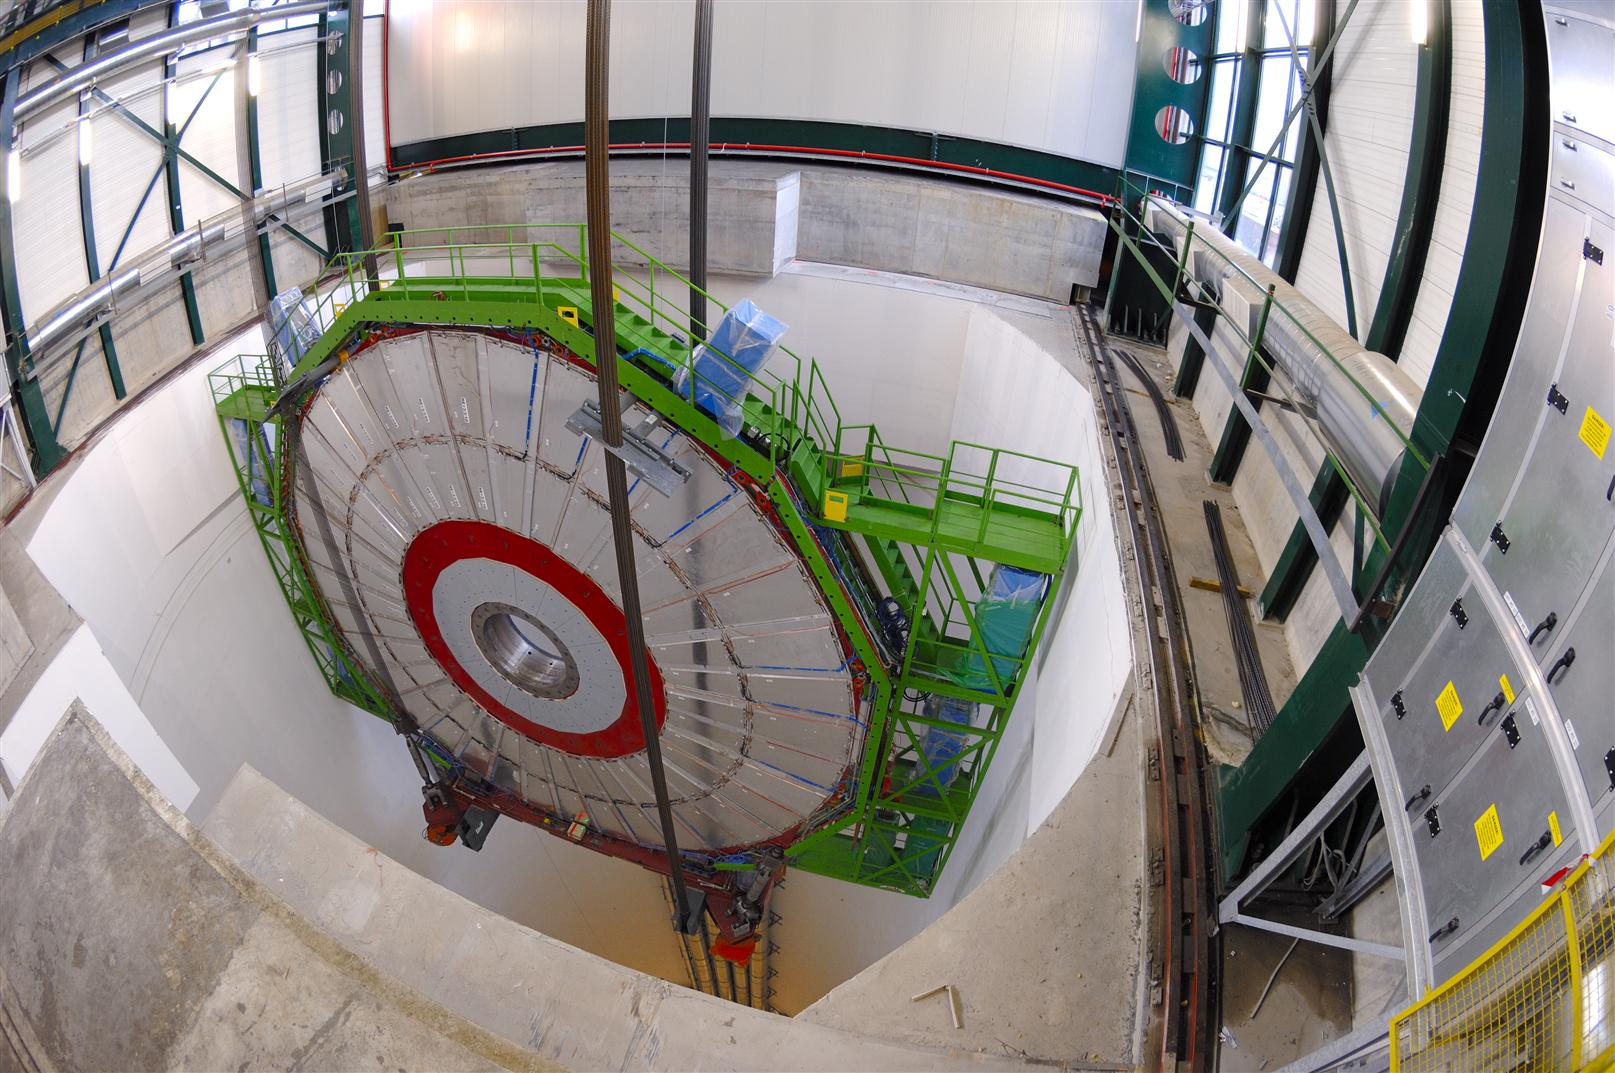
\includegraphics[width=\marginparwidth]{CMS/slice.jpg}
	\captionof{figure}{Descente d'unr tranche de CMS dans la caverne au point P5.}
	\label{slice}
}

CMS est une détecteur cylindrique de 24m de long et de 14.6 m de diamètre pour une masse de plus de 16000 tonnes (cf.fig\ref{cmsexploded}). Il est composé d'une succession de sous-détecteurs concentriques; En partant du centre verss l'extérieur :
\begin{itemize}[label=$\bullet$]
	\item \textbf{Le trajectographe : } C'est le sous-détecteur le plus proche du point d'intéraction. Il permet de reconstruire la trajectoires des particules chargées.
	 \item \textbf{Le calorimètre électromagnètique (ECAL\footnote{Pour Electromagntic CALorimeter.}): Il permet de mesurer l'énergie des photons et des électrons.}
	 \item \textbf{Le calorimètre hadronique (HCAL\footnote{Pour Hadronc CALorimeter}): Il permet de mesurer l'énergie des hadrons.}
	 \item \textbf{L'aimant supr-conducteur : } Il produit un champ de 3.8T est permet de courber la trajectoire des particules chargées.
	 \item \textbf{Les chambres à muons : } Elles permettent d'identifier reconstruire la trajectoire et mesurer l'énergie des muons. 
\end{itemize}
Chaque composant de CMS fera l'objet d'une description plus détaillé dans les paragraphes suivants.

\subsection{Système de coordonnées conventionnel}
Le système de coordonné utilisé dans CMS est un repère cartésien $\left(O,\vec{x},\vec{y},\vec{z}\right)$ où $O$ est l'origine du repère est coîncide avec le point nominal d'interaction (IP) qui est le centre du détecteur. Le système de coordonnée qui suit la convention de la main-droite est determiné par l'axe $z$ qui est défini comme étant parallèle et dans la même direction que le faisceau allant dans le sens anti-horaire. L'axe $x$ pointe vers le centre du collisionneur LHC. L'axe $y$ est orthogonal au plan $xz$ est pointe vers le haut. CMS possédant une symmètrie cylindrique, le repère $\left(O,\vec{r},\vec{\theta},\vec{\phi}\right)$ est souvent utilisé. $r$ correspond à la distance entre le an perpendiculaire à l'axe du faisceau (appelé plan tranverse) passant par le point considérer et l'origine du repère $O$; $\theta$ est mesuré par rapport à l'axe $\vec{x}$ dans le plan $xy$ (angle d'émission par rapport à l'axe du faisceau) et l'angle polaire $\phi$ est définit par rapport à $z$.

Un troisième type de coordonnées, utilisant le fait que les particules produite au LHC sont relativistes, est également utilisé.
En décomposant l'impulsion de la particule en une composante transverse et longitudinale (pr rapport au faisceau)
\begin{equation}
p=p_{T}+p_{L}=\sqrt{p_{x}^{2}+p_{y}^{2}}+p_{z}
\end{equation}
D'où :
\begin{equation}
( E/c)^{2}=(mc)^{2}+p^{2} (E/c)^{2}-p_{L}^{2}=(mc)^{2}+(p_{T})^{2}
\end{equation}
qu'il est possible de réécrire comme :
\begin{equation}
\left( E/c \right)=\sqrt{\left( mc \right)^{2}+p_{T}^{2}}\cosh(y), p_{L}=\sqrt{\left( mc \right)^{2}+p_{T}^{2}}\sinh(y)
\end{equation}
avec $y$ un paramètre appellée rapidité est égale à:
\begin{equation}
y=\arctan\left(\frac{p_{l}c}{E}\right)=\frac{1}{2}\log\left(\frac{E+p_{l}c}{E-p_{l}c}\right)
\end{equation}
en remarquant que $p_{l}=p_{z}=p\cos(\theta)$ et en faisant le développement de $E=\sqrt{m^{2}c^{4}+p^{2}c^{2}}$
\begin{equation}
y=\frac{1}{2} \log\left(\frac{E+p_{l}c}{E-p_{l}c}\right)=\frac{1}{2}\log\left(\frac{\cos^2 \theta/2+m^{2}c^{2}/4p^{2}+\cdots}{\sin^2 \theta/2+m^{2}c^{2}/4p^{2}+\cdots}\right)\backsimeq-\log\tan\left(\frac{\theta}{2}\right)=\eta
\end{equation}
On utilise donc le repère $\left(O,\vec{r},\vec{\theta},\vec{\eta}\right)$ pour décrire la géométrie de CMS.
\begin{sidewaysfigure}
	\centering
	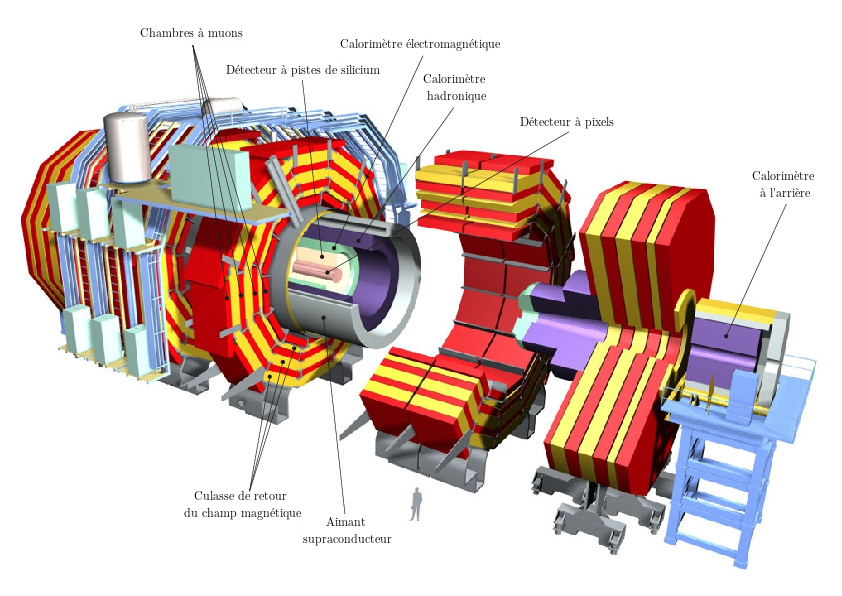
\includegraphics[width=0.8\textwidth]{CMS/cms.png}
	\caption{\label{cmsexploded}Vue éclatée du détecteur CMS.}
\end{sidewaysfigure}
\section{Les sous detecteurs de CMS}
\subsection{Le trajectographe}
Le trajectographe de CMS (cf.fig\ref{trajectographe}) est le détecteur le plus proche du faisceau et fu point de collision.Il a pour but de reconstruire les traces des particules chargées issues des collisions grâce à des suites d'impacts enregistrés par les couches du détecteur. La trace reconstruite permet de déterminer la charge et l'impulsion de la particule associée. En effet, une particule de charge $q$ qui se déplace dans un champ magnétique subit une force donné par la formule de Lorentz. La trajectoire de la particule dans le cas d'un champ magnétique d'intensité $B$ est hélicoïdale, de rayon $R_{c}$. Il est ainsi possible dans déduire l'impulsion transverse :
\begin{equation}
p_{T}=qBR_{c}
\end{equation}
En prenant les positions selon r des hits, il est possible d'en déduire l'angle $\theta$, angle entre la trajectoire de la particule est le faisceau et donc de calculé l'impulsion totale:
\begin{equation}
p=\frac{p_{T}}{\sin\theta}
\end{equation}
\begin{figure}[ht!]
	\centering
	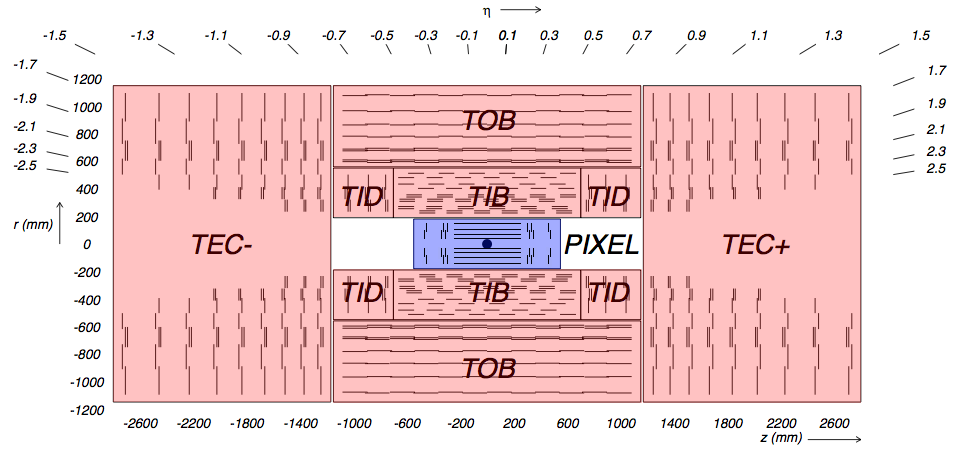
\includegraphics[width=0.9\textwidth]{CMS/tracker.png}
	\captionof{figure}{Schéma du trajectographe de CMS. Chaque trait reprèsente un mosule du détecteur. Les lignes double correspondent à des modules mis dos à dos est produise des hits dit stéréo. Le détécteur à pistes est composé de quatre sous-détecteur: Les tonneaux interne (TIB), les tonneaux externe (TOB), les disques interne (TID) et les bouchons (TEC).}
	\label{trajectographe}
\end{figure}

Le trajectographe est composé de deux sous-détecteurs : le détecteur à pixels et le trajectographe à micro-piste de silicium.
\subsubsection{Le détecteur à pixels}
Le détecteur à pixels de CMS à récemment était remplacé afin de garder un tracking performant à des luminositées au dessus de $2\times10{34}cm^{-2}s^{-1}$ et avec un pile-up de plus de $50$. Ce remplacement à eu lieu du 28 février au 7 mars durant l'arrêt technique de hivernal prolongé (EYETS). Le nouveau détecteur à pixels se compose d'un tonneaux constitué de quatre couche de détection (BPIX) à des distances du faisceau $r=3.0$cm,6.8cm,10.2cm et 16cm et d'une longueur de 548.8mm et de trois bouchons (FPIX) situé à $\pm$29.1cm,$\pm$39.6cm et $\pm$51.6cm pour une couverture radial allant de 4.5 à 16.1cm . Une comparaison entre l'ancien détecteur à pixel et le nouveau est donné fig.\ref{pixel}.

	\begin{figure}[ht!]
	\subfloat[Ancien détecteur à pixel (bas) et nouveaux (haut)]{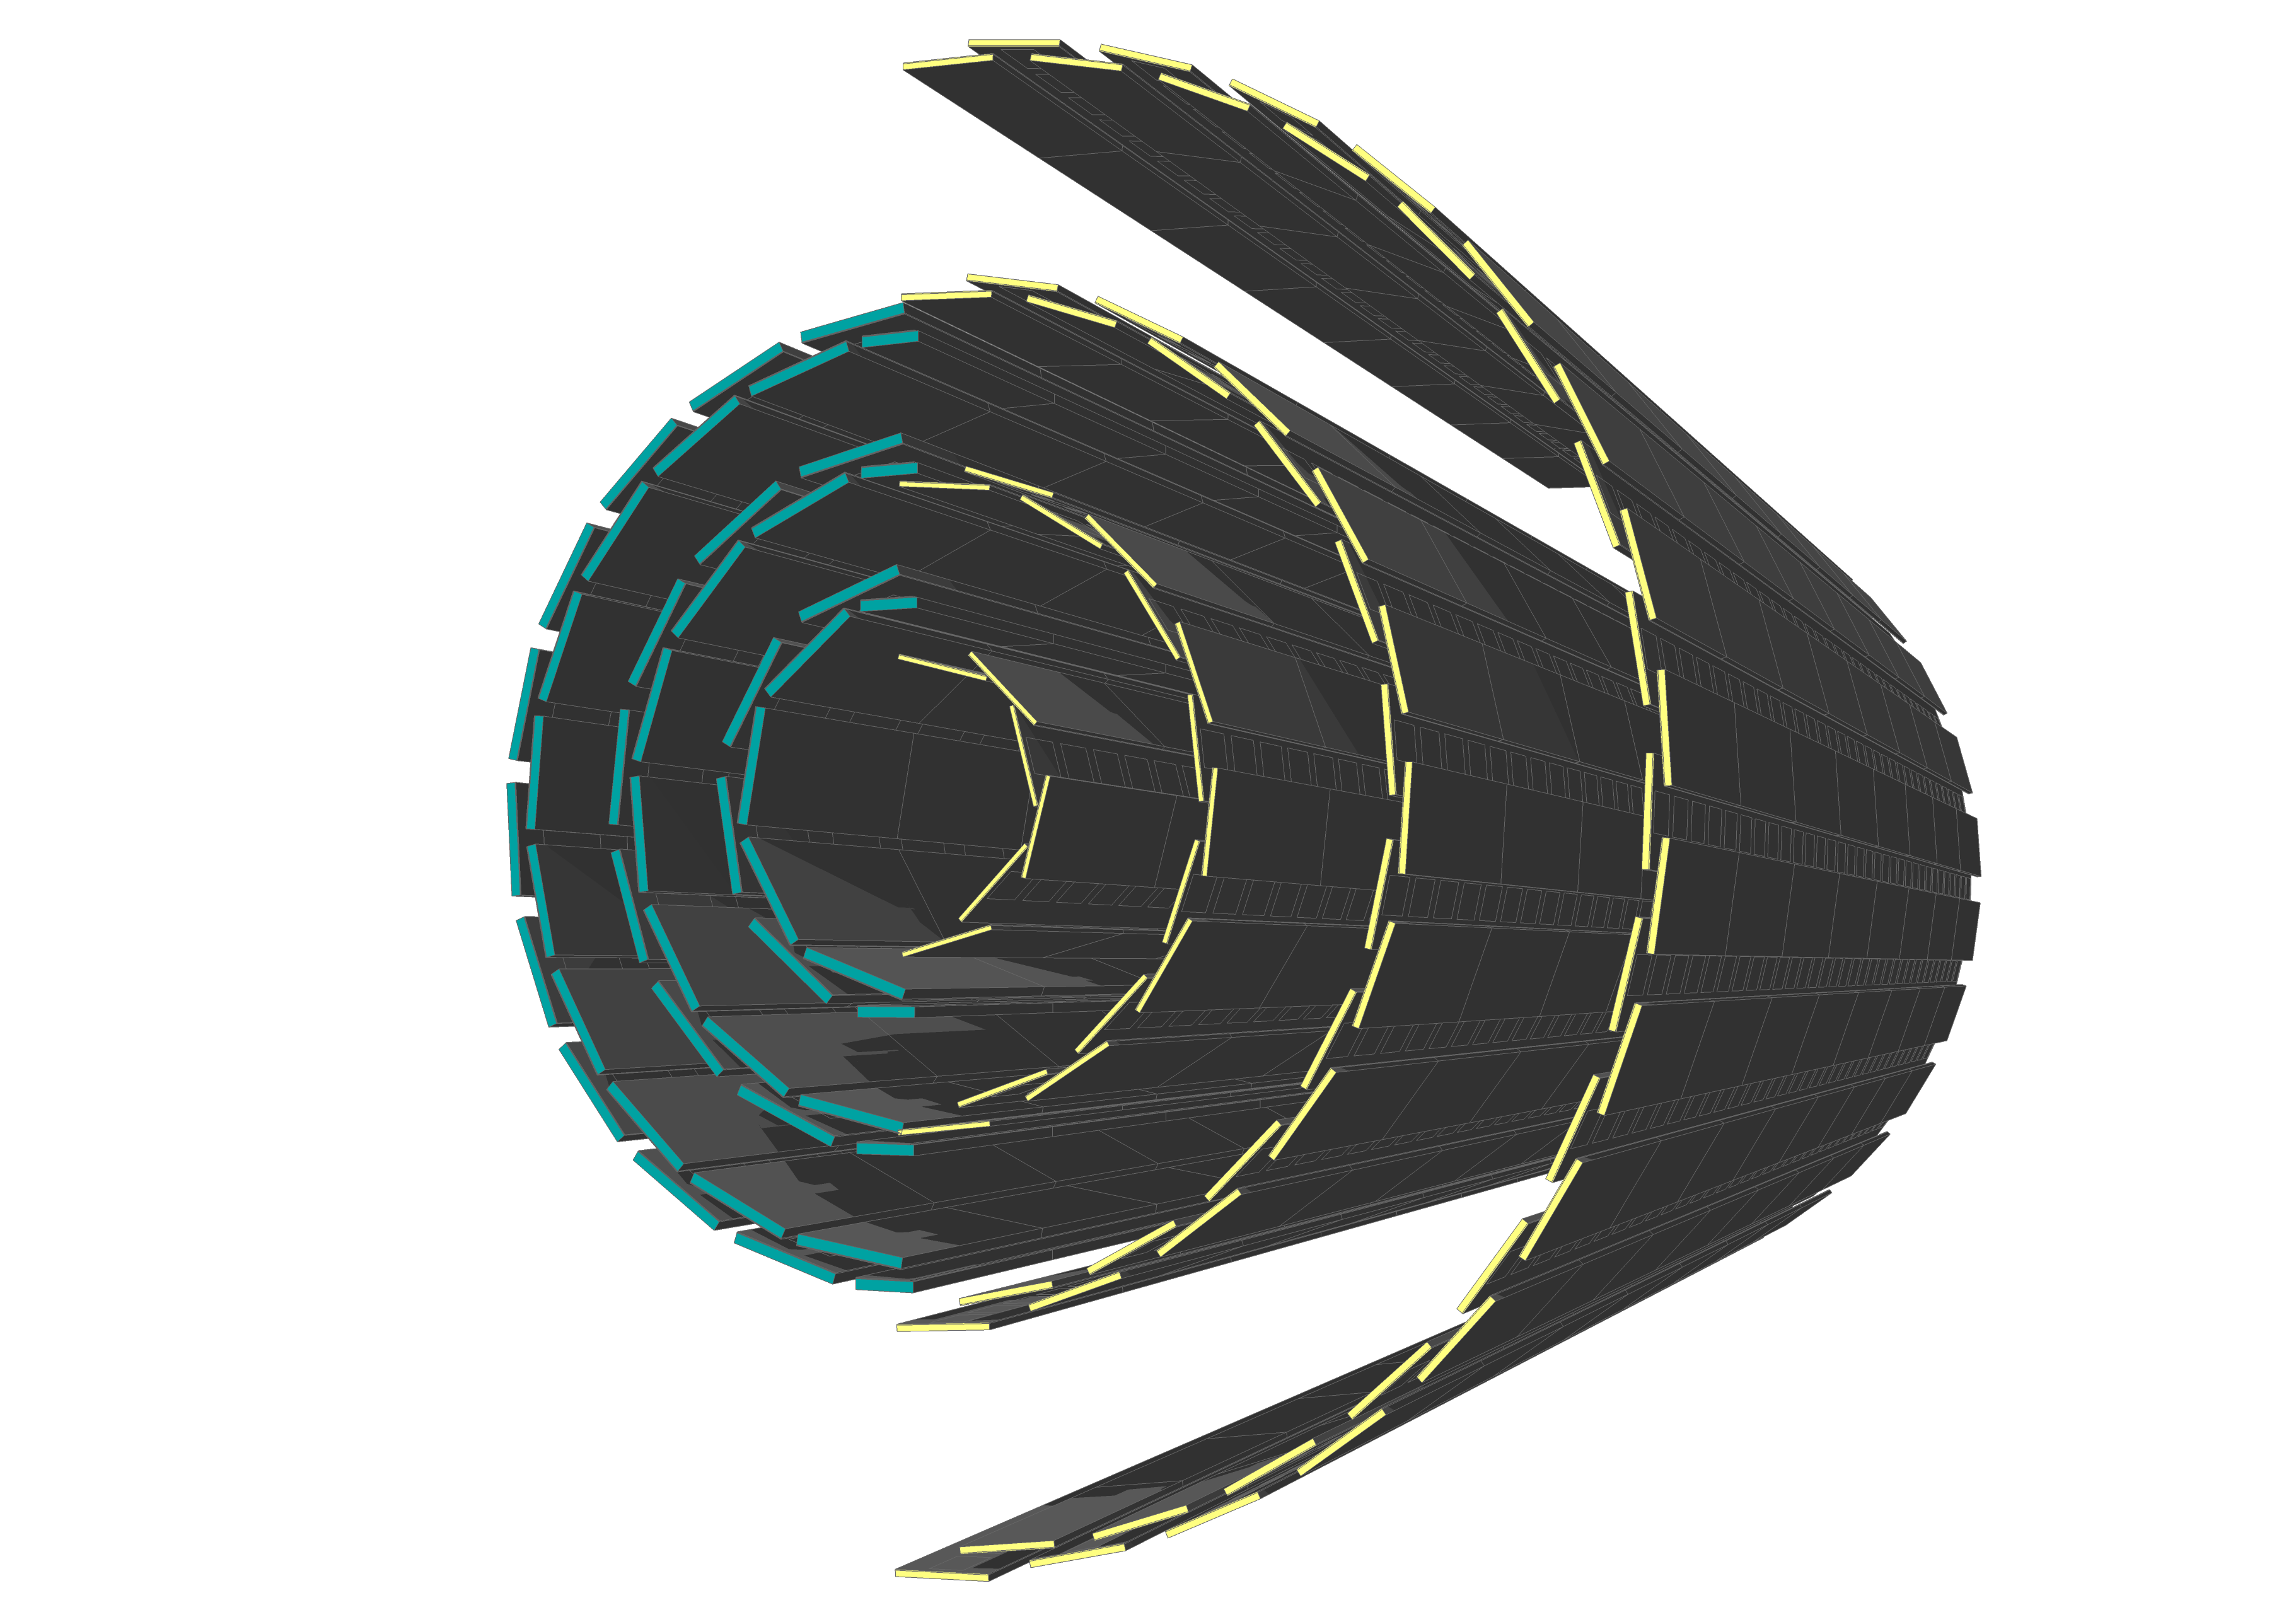
\includegraphics[width=.45\linewidth]{CMS/pixel.png}}
	\hfill
	\subfloat[ Vue oblique-transverse comparant les couche des tonneaux de 'ancien (gauche) et le nouveau déecteur]{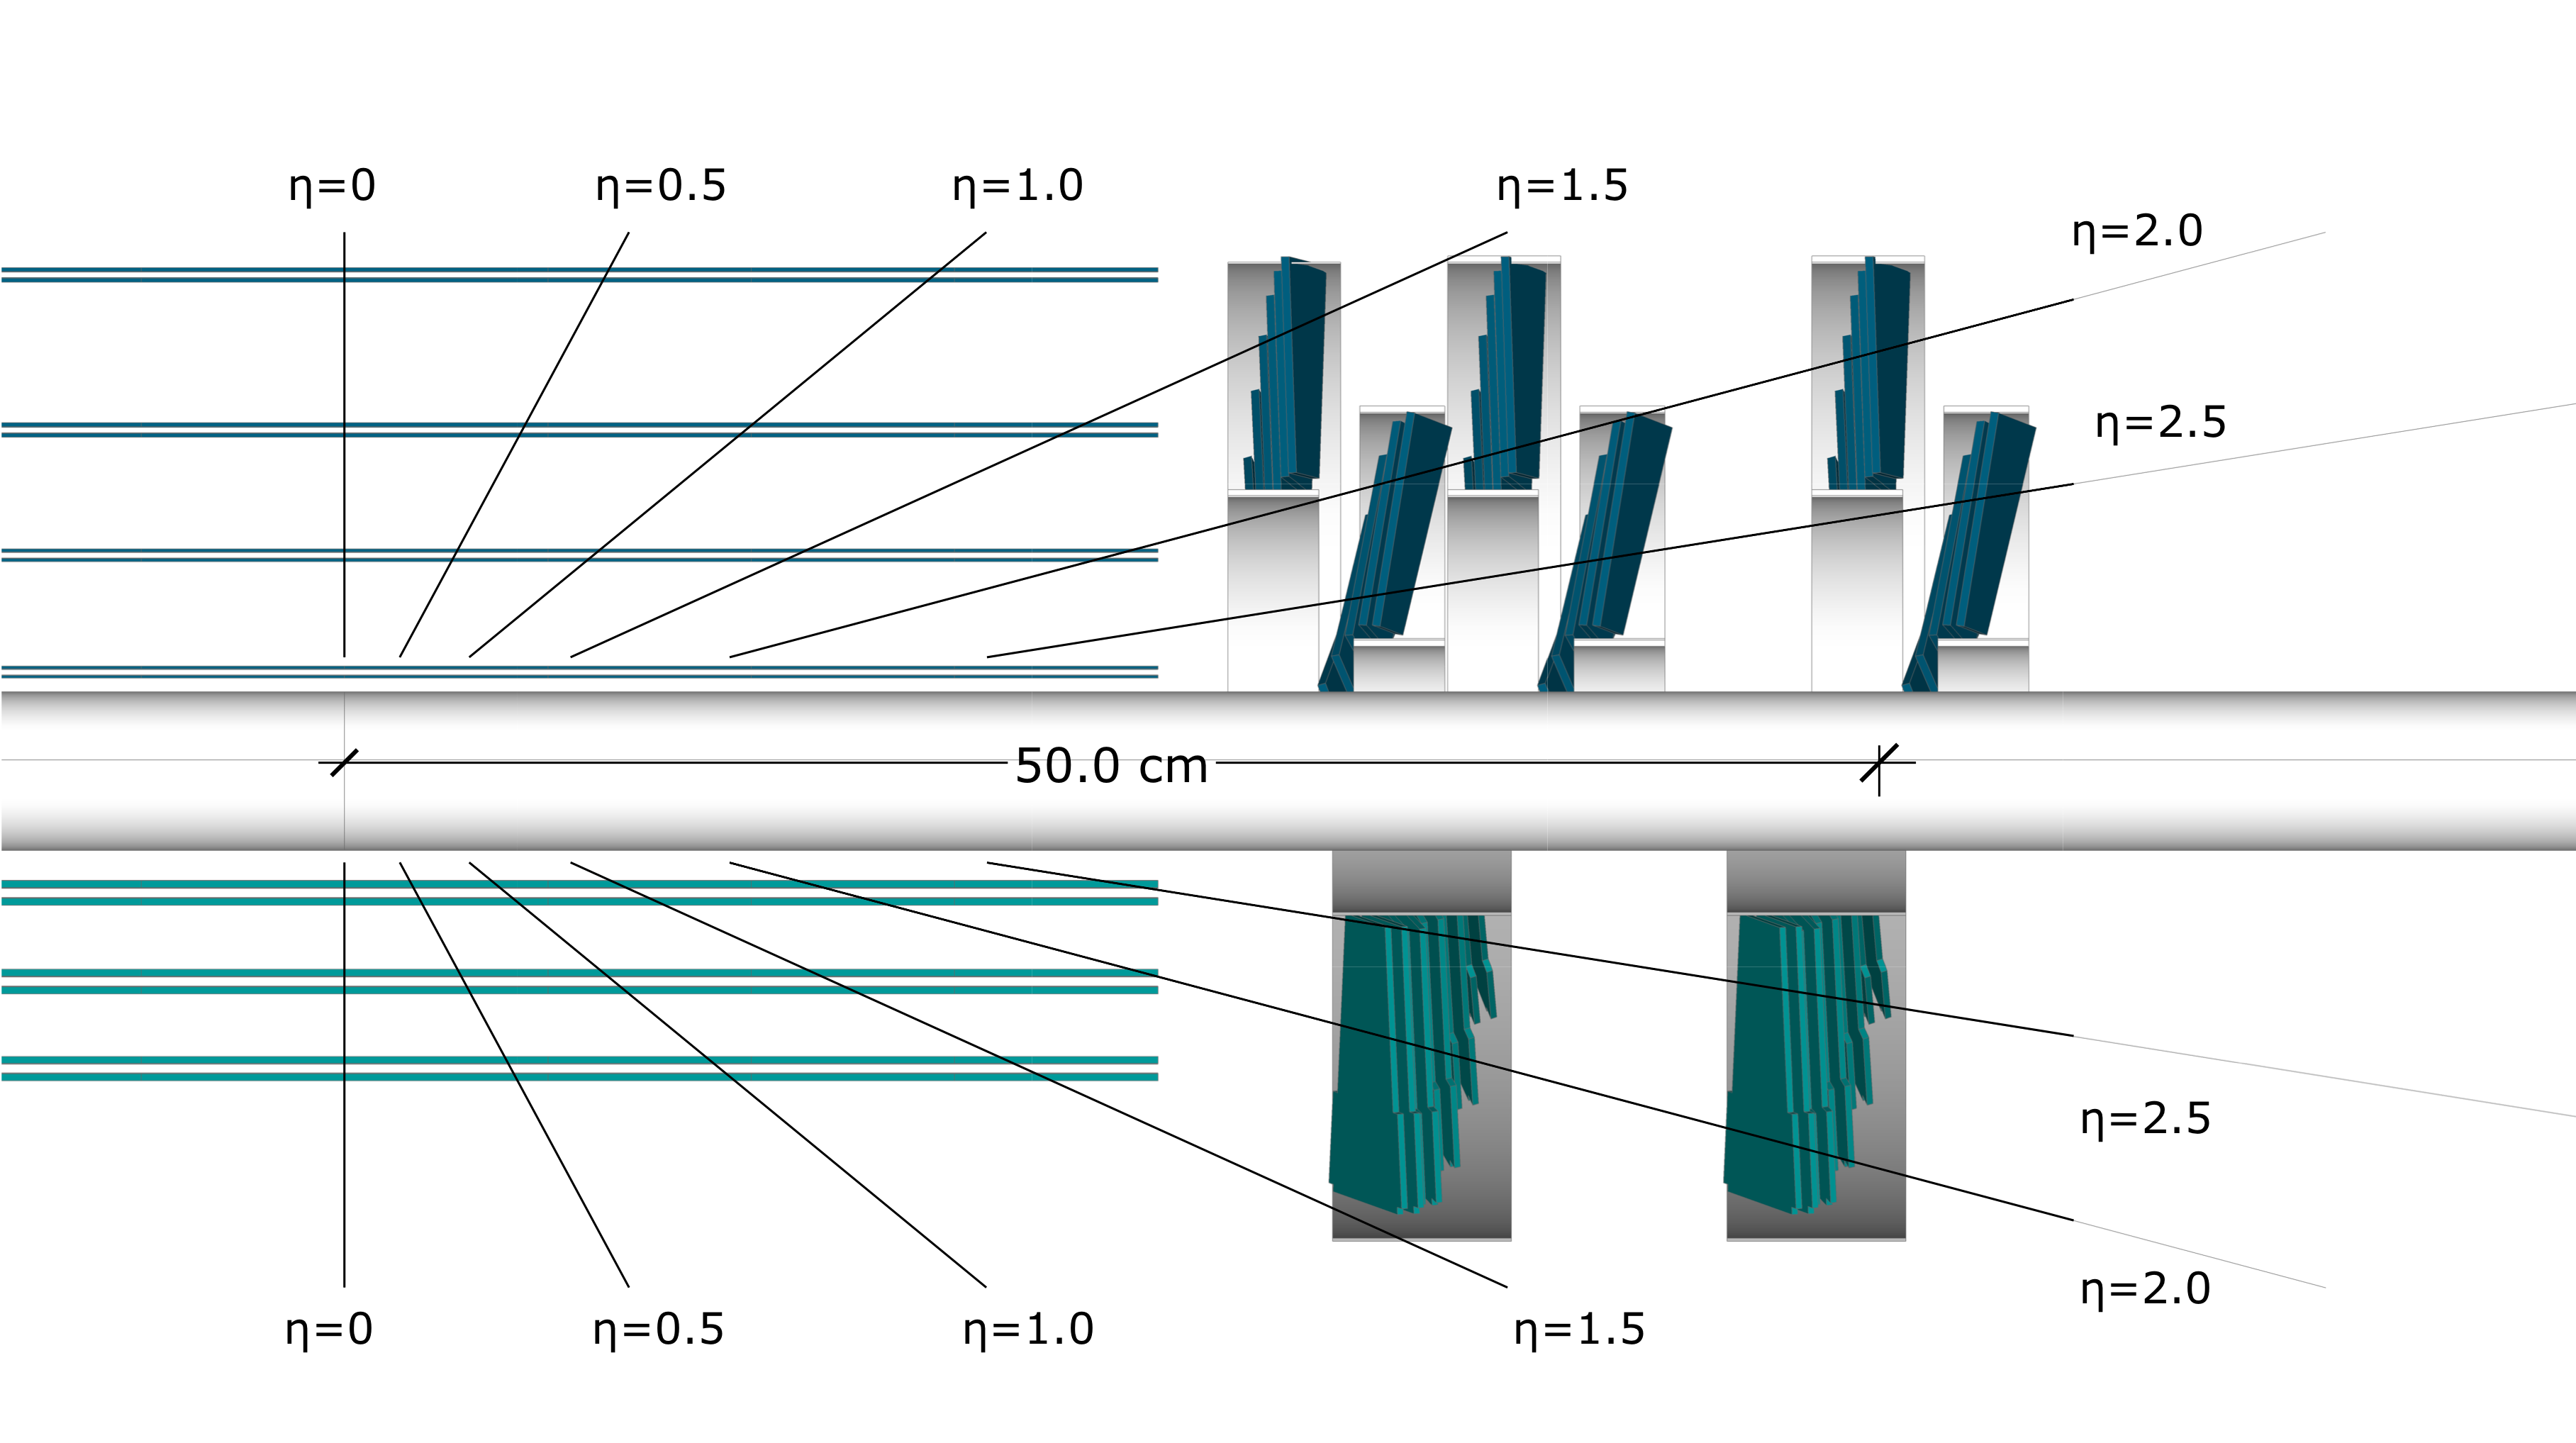
\includegraphics[width=.45\linewidth]{CMS/pixel2.png}}
	\caption{Comparaison entre le nouveau et l'ancien trajectographe à pixels.}
	\label{pixel}
\end{figure}

L'ajout d'une quatrieme couche de détection dans le barrel assure une redondance lors de la reconnaissance de pattern et permet de réduire le fake rate lors de pile-up important. Il assure également une sécurité au cas où la couche la plus proche du point d'interaction viendrait à se déterioré plus vite que prévu.Cependant, elle augmente le budget matériel du détecteur, il a donc été nécessaire de repenser le support et les services afin d'être plus léger. 
Un nouveau système de refroidessement au $CO2$ ainsi que la déplacement des système passif (connectique plaques d'electronique) hors d'une volume de tracking à également été effectué (cf.fig\ref{pixel2}).

\begin{figure}[ht!]
	\centering
	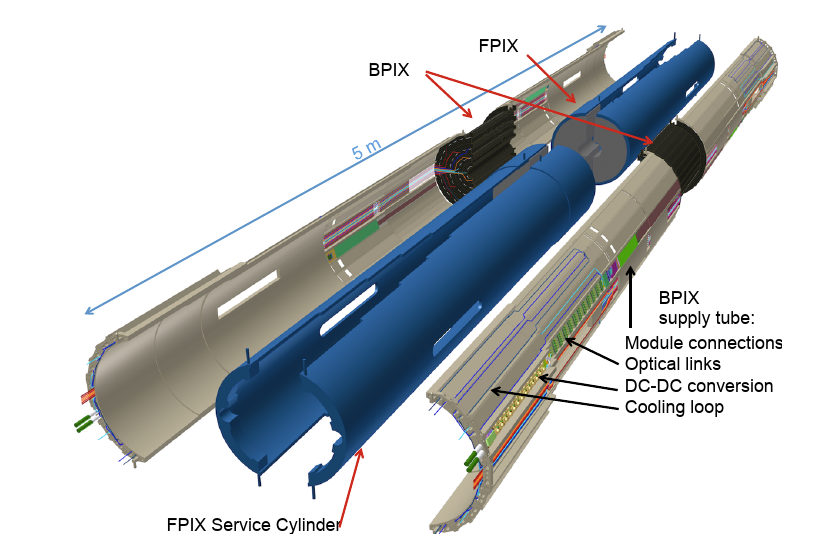
\includegraphics[width=0.55\textwidth]{CMS/pixel3.png}
	\captionof{figure}{Vue explosée du nouveau détecteur à pixels. La figure montre les positions des différentes partitions FPIX et BPIX ainsi que leur cylindres contenant leur service respectifs. Les services nécessaires au détecteur (connectiques, fibre optique, convertisseur DC-DC sont situés à haut $\eta$, hors du volume de tracking.)}
	\label{pixel2}
\end{figure}

Ce détecteur contient plus de 97 millions de pixels (79pour les BPIX et 18 pour les FPIX) mesurant $100\times150\mu m$ de section et $250\mu m$ d'épaisseur. Ces pixels sont regroupés en module (1184 pour BPIX et 672 pour FPIX) (cf.fig\ref{module}) de 66560 pixels  (8$\times$ 2 ROCs) d'une épaisseur de $75\mu m$ pour la premiere couche du BPIX et $250\mu m$ pour les reste du BPIX et FPIX.

	\begin{figure}[ht!]
	\centering
	\subfloat[Module pour les couches 2 à 4 des BPIX et des FPIX (gauche) et de la couche 1 de BPIX (droite)]{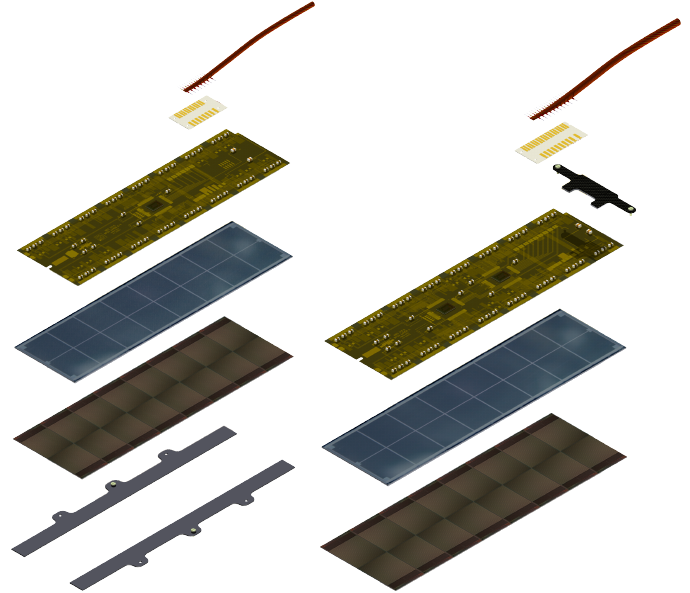
\includegraphics[width=.46\linewidth]{CMS/module.png}}
	\subfloat[Schéma de l'électronique de lecture d'un module]{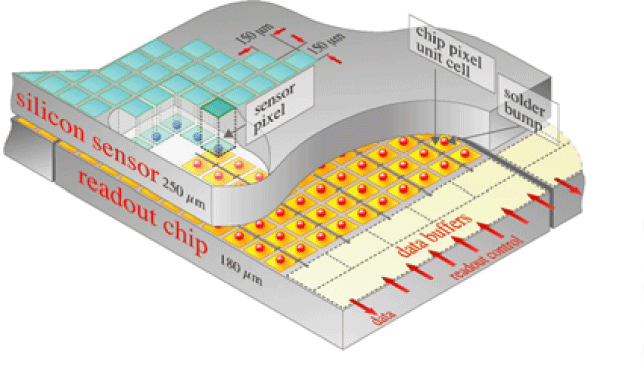
\includegraphics[width=.46\linewidth]{CMS/module2.png}}
	\caption{Modules de pixels.}
	\label{module}
\end{figure}
\subsubsection{Le détecteur à pistes}
Le détecteur à pistes mesure 5.5m de long pour 2.4m de diamètre pour une aire active de 198m2 et est le plus grand détecteur au silicium jamais construit.Il comporte en tout 15148 modules pour un totale de 9.3 millions de pistes lus par 76000 chips électroniques. Il peut être décomposé en quatre sous-détecteurs :

\begin{itemize}[label=$\bullet$]
\item \textbf{Le tonneau interne}Le tonneau interne (TIB) (cf.fig\ref{TIB}) pour  \textit{Tracker Inner Barrel} est composé 2724 modules répartis en quatre couches. Chaque couche se compose de pistes de silicium d'une épaisseur de $320 \mu m$ avec un pas de $80$ à $120\mu m$ pour les deux premières et 2 derniere couches respectivement. Elles sont orientés parallèlement au faisceau. Les deux première couches sont composées de modules dits "stéréos" qui sont la juxstaposition de deux modules collés l'un l'autre avec un angle de $100mrad$ entre les deux. Celui permet d'avoir une résolution de $23$ à $34\mu m$ dansle plan transverse et de $230\mu m$ dans le plan longitudinale. Il s'étend entre 25 et 52 en rayon et $|z|<65cm$.

\item \textbf{Les disques internes} (TID) (cf.fig\ref{TID}) pour \textit{Tracker Inner Disk} sont composés de trois disques parallèles qui vont jusqu'à $75cm<|z|<110cm$.Chaque disques est composé de trois anneaux concentriques. Les 816 modules sont composés de strips d'une épaisseur$320\mu m$ de orienté radialement pour un pas compris entre $81\mu m$ et $158\mu m$. Comme pour le TIB, les deux premier modules sont "stéréos".
\marginpar
{
	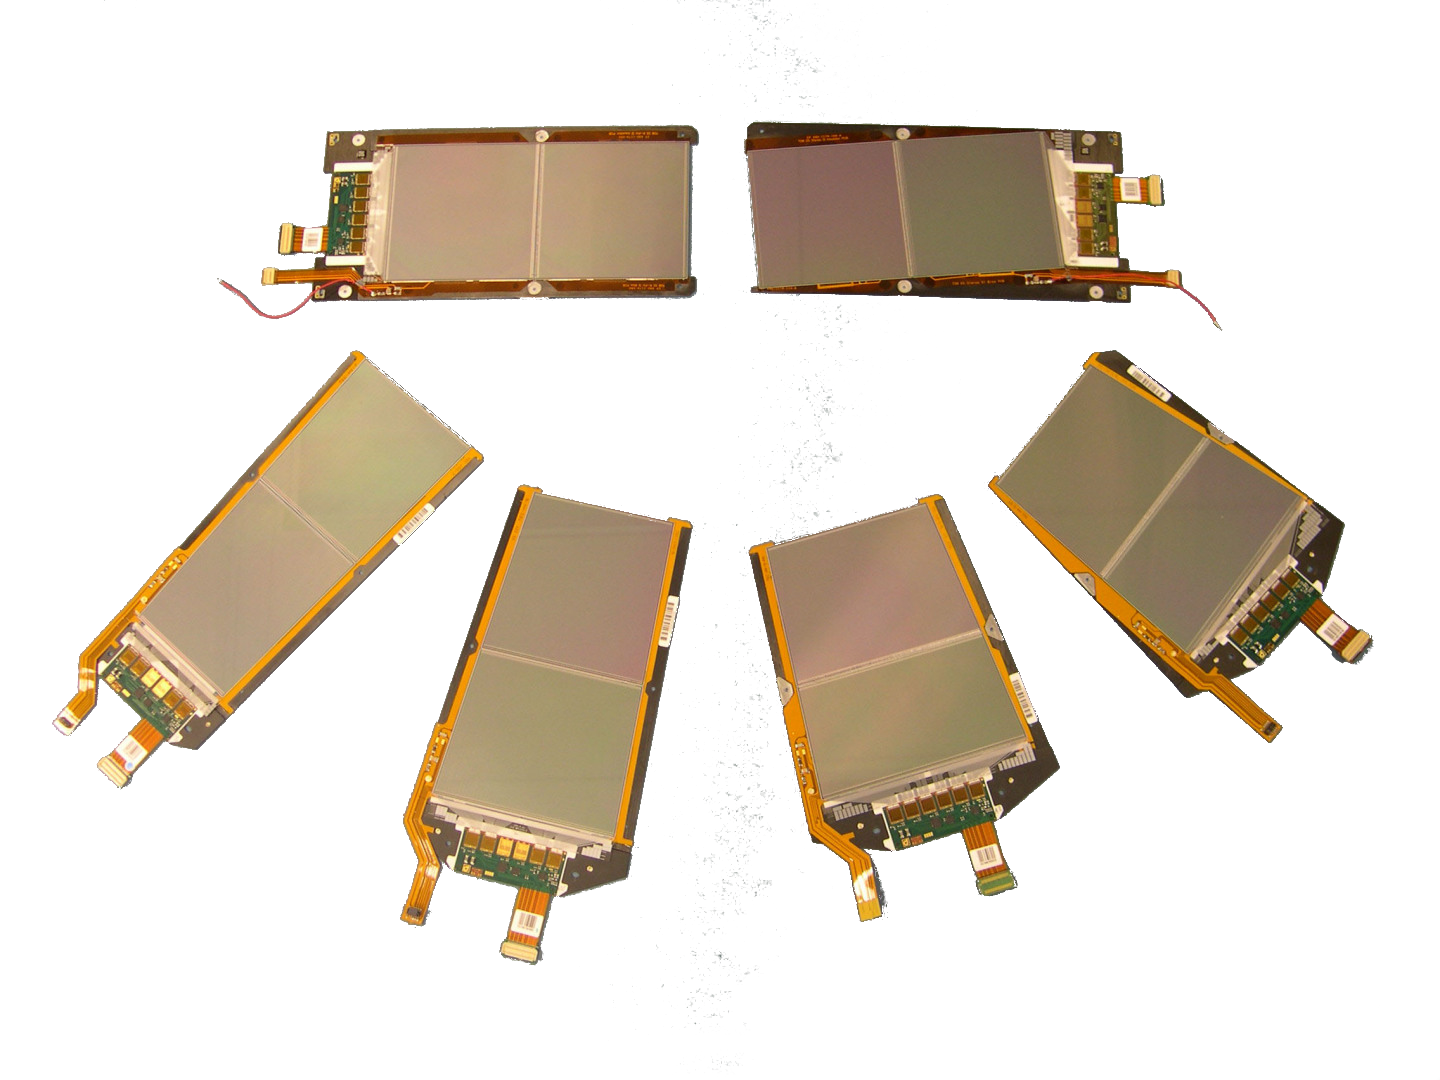
\includegraphics[width=\marginparwidth]{CMS/TOB_TEC.png}
	\captionof{figure}{Différents modules utilisés pour la construction de TOB et TEC.}
	\label{TOB_TEC}
}
\item \textbf{Le tonneau externe } (TOB) (cf.fig\ref{TOB})pour \textit{Tracker Outer Barrel} enroule les TIB et TID pour couvrir un espace entre 60 et 100cm en rayon et $|z|<110cm$. Il est composé de 5208 modules (cf.fig\ref{TOB_TEC}) de pistes orientés parallement au faisceau et de pas compris entre 122 et 183 $\mu m$. Ces modules sont répartis en six couches dont les deux dernieres sont "stéréos". L'épaisseur de ces modules est de $500\mu m$   

\item \textbf{Les bouchons }(TEC) (cf.fig\ref{TEC}) pour \textit{Tracker End-Cap} sont composés de neuf disques chacun, composée de 4 à 7 anneaux concentriques. Il couvre 25-110cm en rayons et 120-275cm en $|z|$. Les deux premier disques ainsi que le cinquieme sont "stéréos". Les trois premier anneaux sont composés de 2512 modules (cf.fig\ref{TOB_TEC}) d'épaisser 320$\mu m$ et de pas inter-pistes compris entre 81 et 158 $\mu m$. Les quatres anneaux suivant, composés de 3888 (cf.fig\ref{TOB_TEC}) en tout d'épaisser $500\mu m$ de pas inter-strip 113-172$\mu m$
\end{itemize}
	\begin{figure}[ht!]
	\centering
	\subfloat[Photo du TIB.]{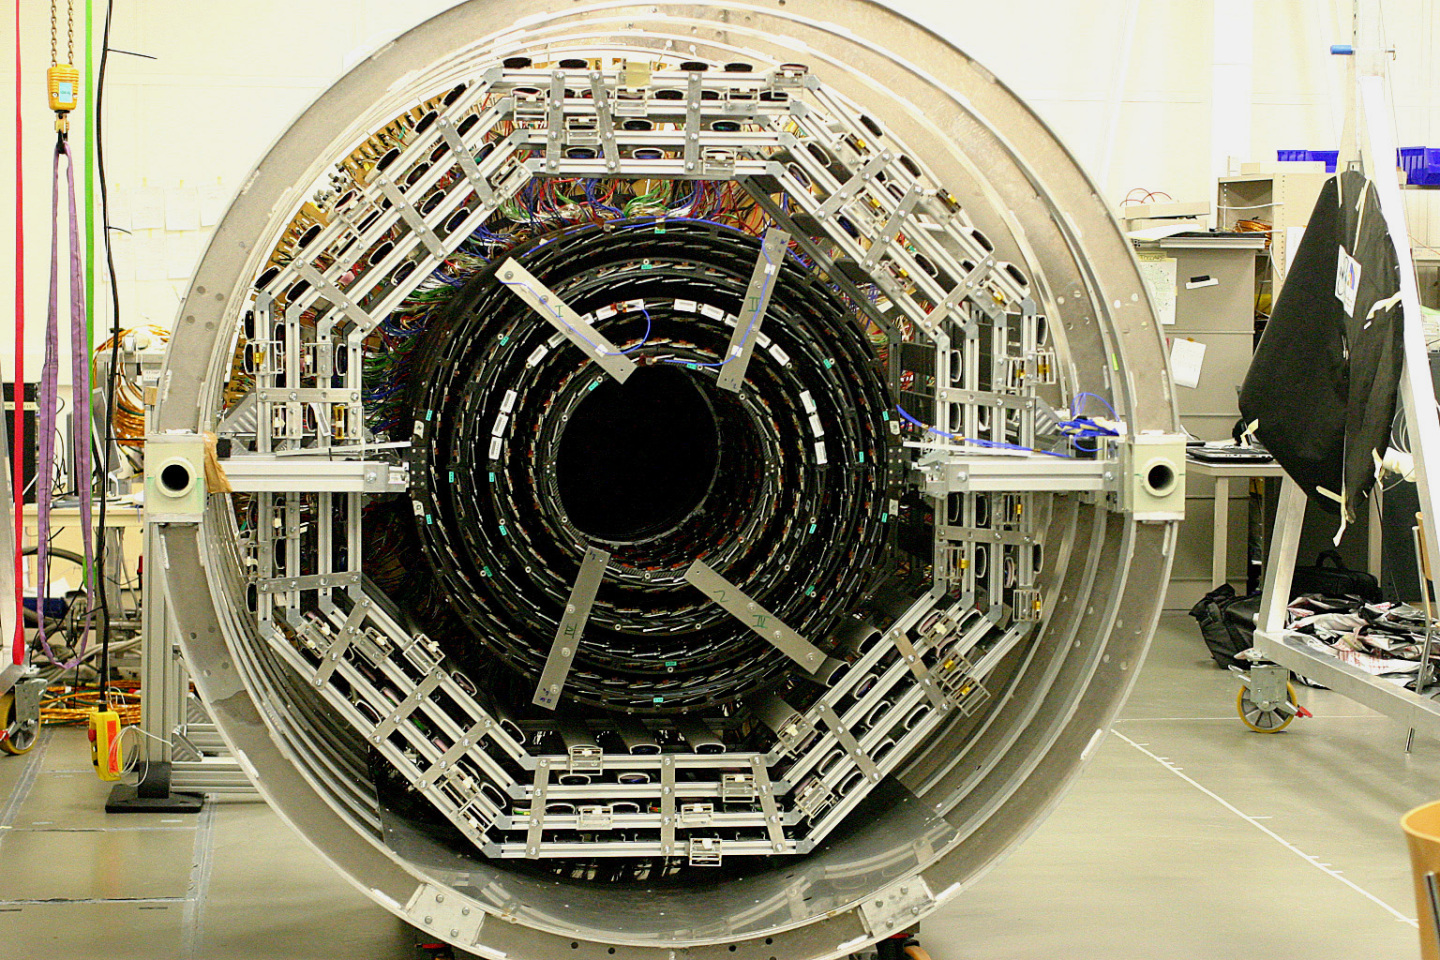
\includegraphics[width=.40\linewidth]{CMS/TIB.jpg}\label{TIB}}
	\subfloat[Photo du TID.]{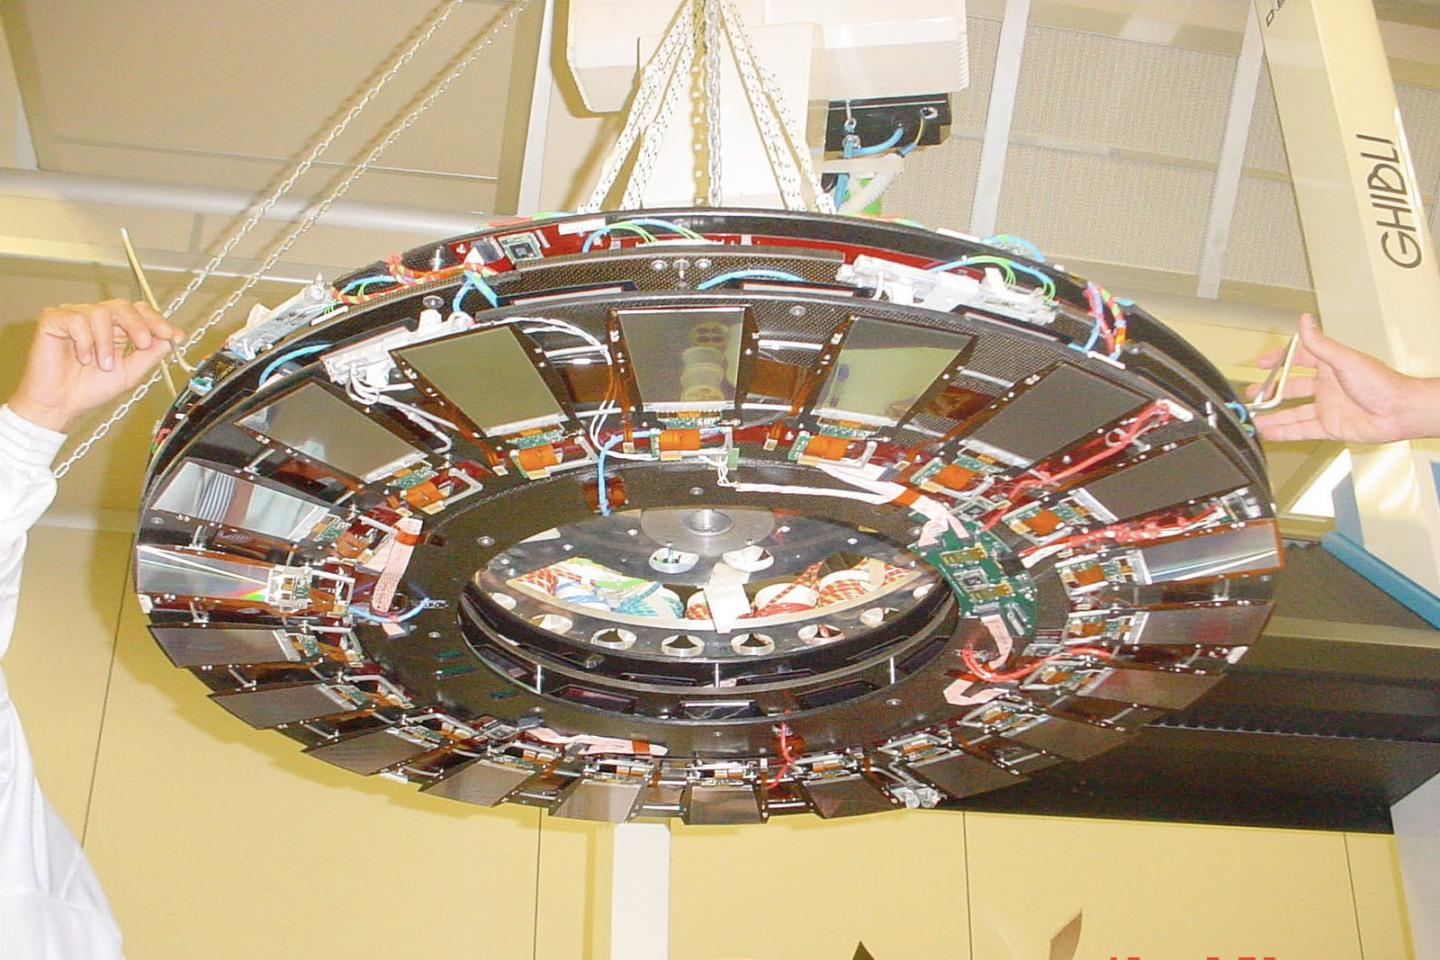
\includegraphics[width=.40\linewidth]{CMS/TID.jpg}\label{TID}}
	\\
	\subfloat[Photo du TOB.]{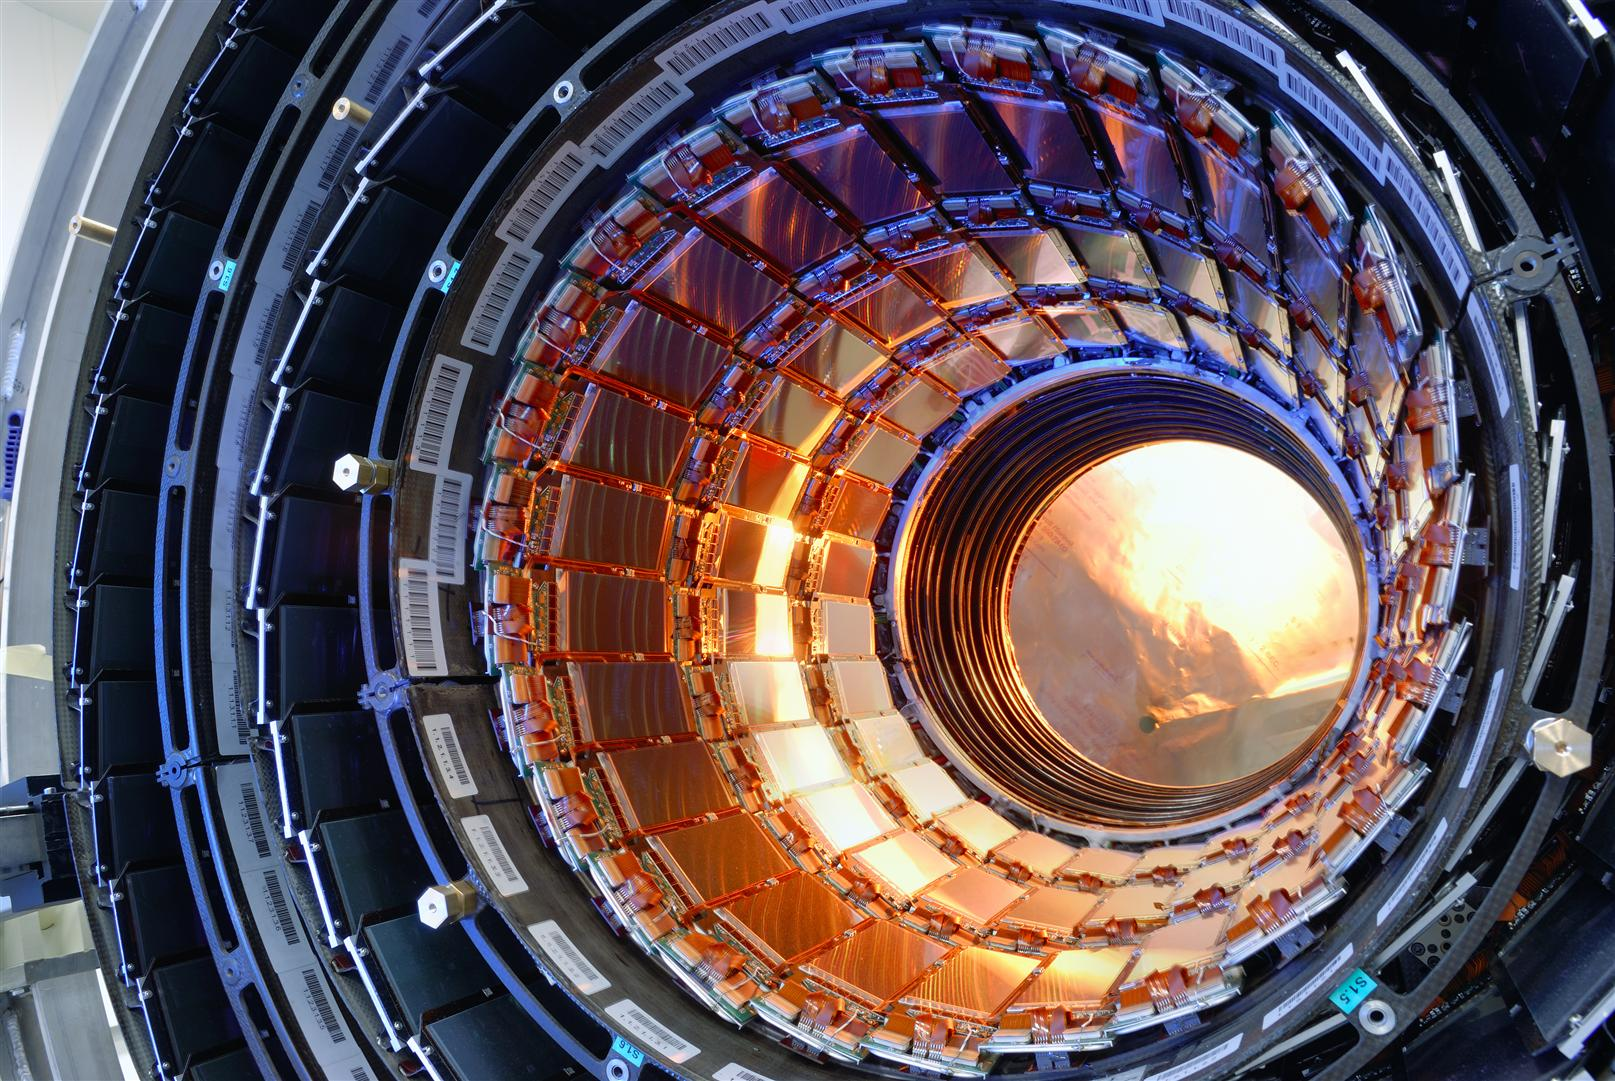
\includegraphics[width=.40\linewidth]{CMS/TOB.jpg}\label{TOB}}
	\subfloat[Photo du TEC.]{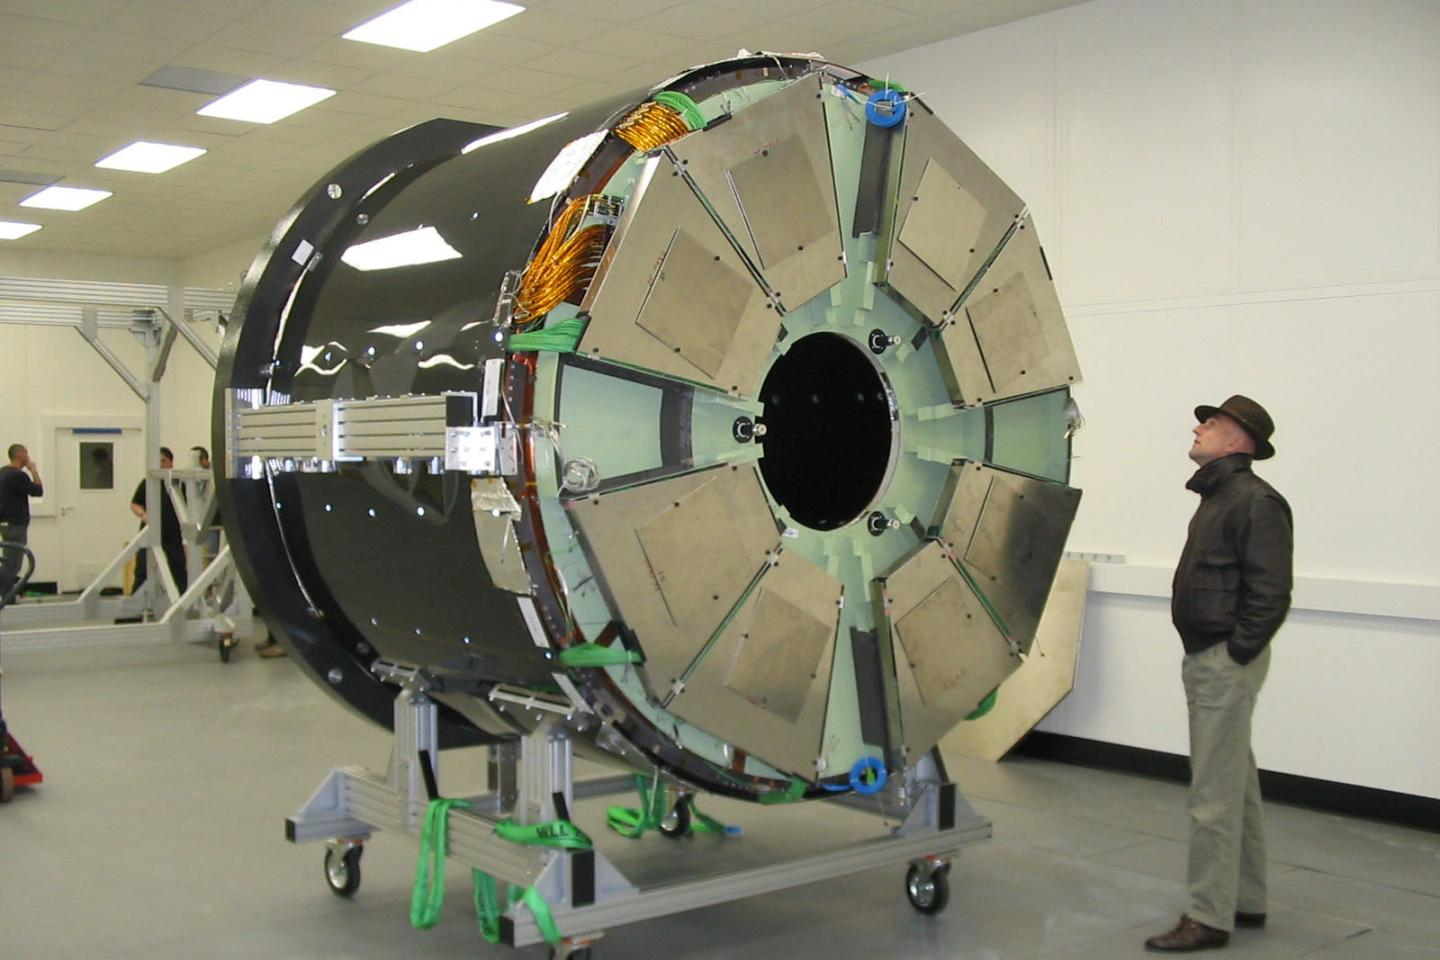
\includegraphics[width=.40\linewidth]{CMS/TEC.jpg}\label{TEC}}
	\caption{Photos des différents composants du détecteur à pistes}
	\label{detecteur}
\end{figure}

\subsection{Le calorimètre électromagnétique}
Le calorimètre électromagnètique de CMS ou (ECAL) pour \textit{Electromagnetic CALorimeter} permet de mesurer l'énergie et la direction des particules réagissant à l'interaction électromagnétique. Ce sont surtout les phtons et les électrons qui seront détectés; ils perdent surtout leurs énergies par des processus radiatifs. La distance caractéristique est donnée par la longueur de radiation $X_{0}$, dépendante du matériaux, définie comme le libre parcours moyen pour le processus de radiaction. Des photons de 100GeV perderent à peu prêt toute leurs énergie dans 20*$X_{0}$.
\begin{figure}[ht!]
	\centering
	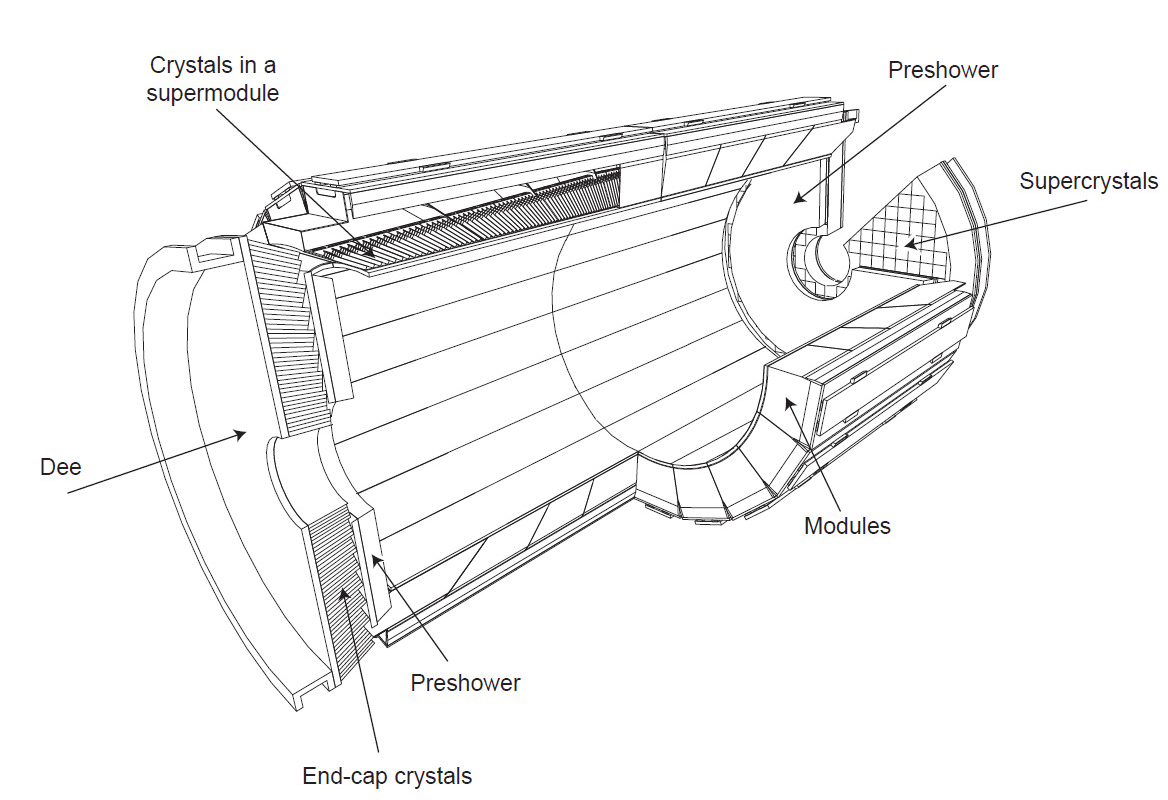
\includegraphics[width=0.90\textwidth]{CMS/ECAL.png}
	\captionof{figure}{Schéma du ECAL de CMS.}
	\label{pixel2}
\end{figure}

\marginpar
{
	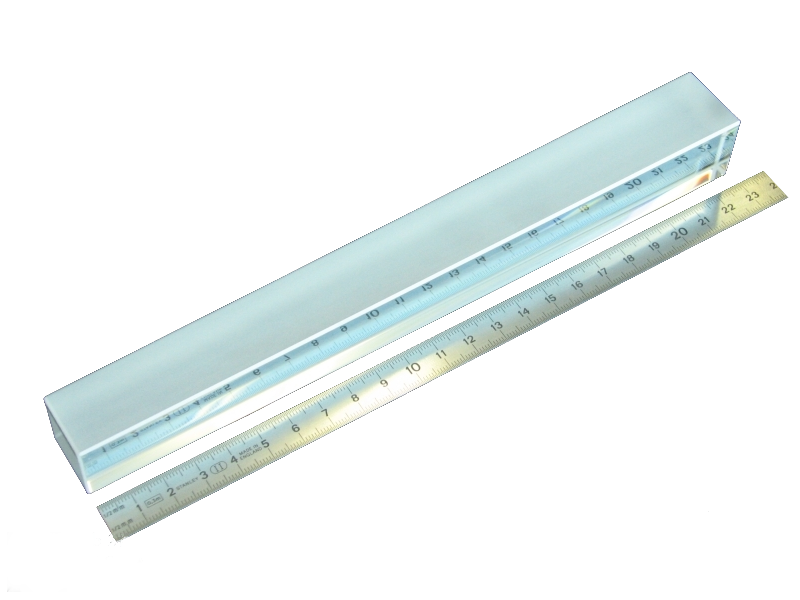
\includegraphics[width=\marginparwidth]{CMS/Crystaux.png}
	\captionof{figure}{Photo d'un crystal de PbWO4.}
	\label{crystaux}
}

	\marginpar
{
	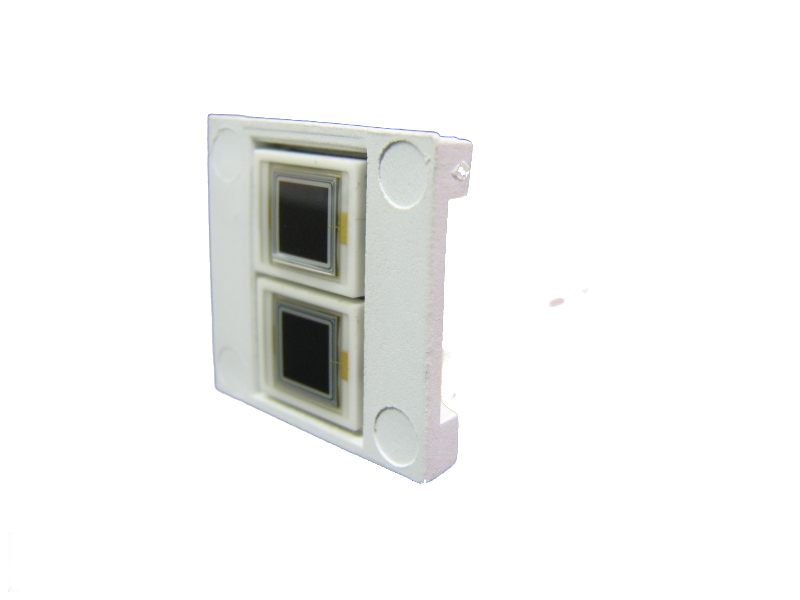
\includegraphics[width=\marginparwidth]{CMS/APD.png}
	\captionof{figure}{Photo d'un groupe de deux APD.}
	\label{APD}
}
Le calorimètre électromagnétique est composé de 75848 cristaux (cf.fig\ref{crystaux}) de PbWO4 (11m3, 92tonnes)et peut se décomposé en trois sous-structures :
\begin{itemize}[label=$\bullet$]
	\item \textbf{Le tonneau} ou EB (cf.fig\ref{EB}) pour \textit{Electronic Barrel} contient 61200 crystaux de tungstate de plomb. Le tonneau est divisé en 36 supermodules couvrant chacun la moitié de la longueur du tonneau. Chaque super-module contient 1700 crystaux de 22*22 mm2 et de longueur 230mmm. Les crystaux sont arrangée de maniere à formée 170-$\eta$ anneaux contenant 360 crystaux chacun. Un crystal couvre environ 1$\degres$ en $\phi$. Le barrel couvre une zone en pseudorapidité de $|\eta|<1.479$. Les photodiodes à avalanches (cf.fig\ref{APD}) (APD) sont utilisées pour détecter la scintillation.
	
	\begin{figure}[ht!]
		\centering
		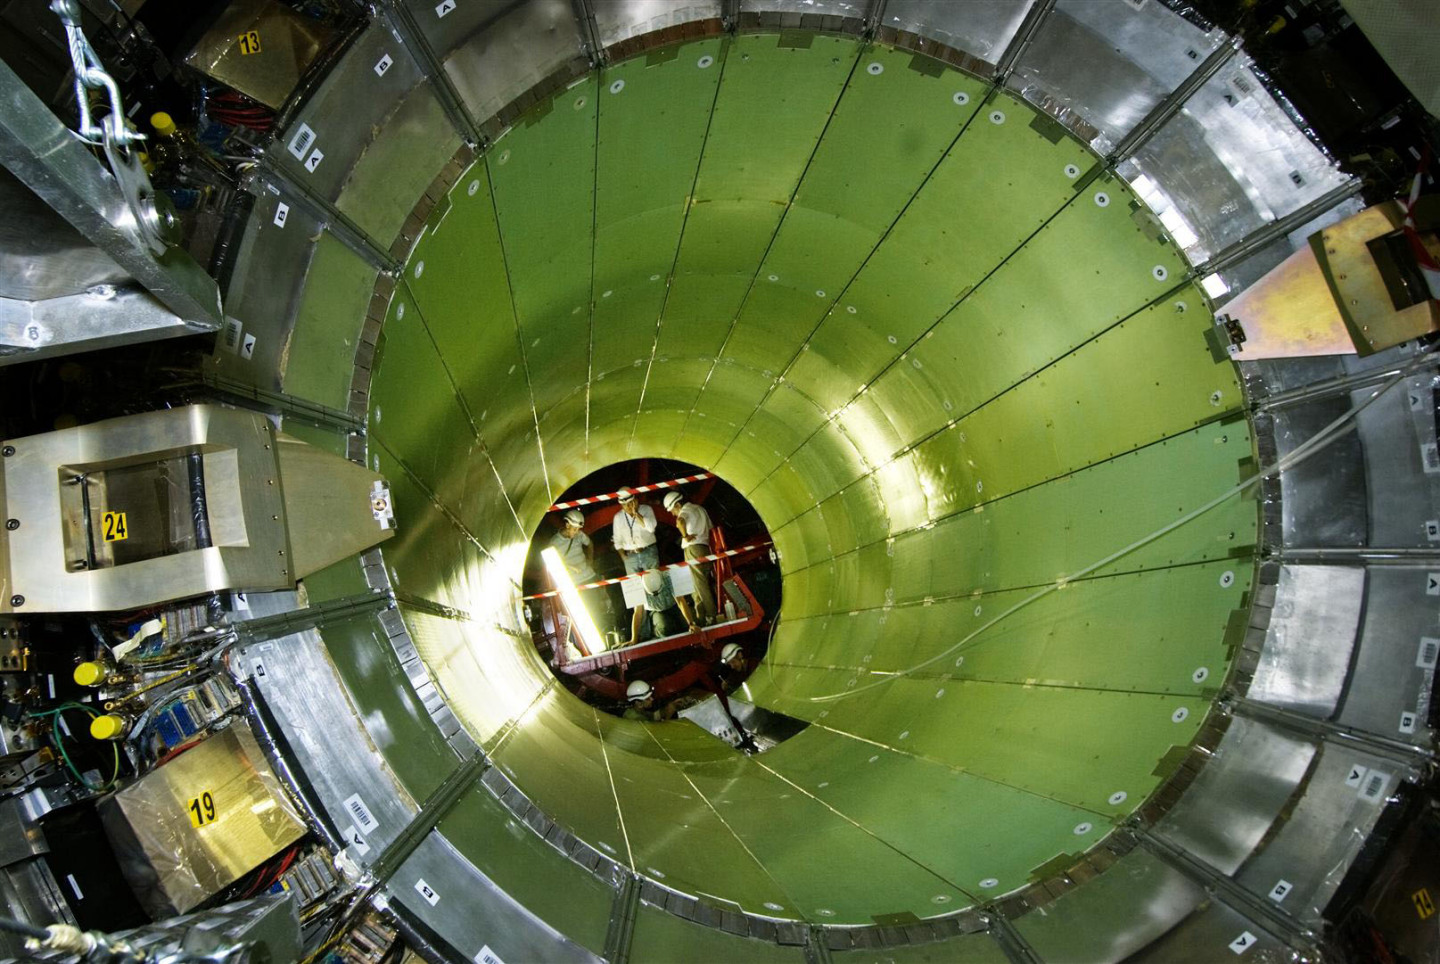
\includegraphics[width=0.55\textwidth]{CMS/EB.jpg}
		\captionof{figure}{Photo du EB.}
		\label{EB}
	\end{figure}
	
	\item \textbf{Les bouchons} (EE) (cf.fig\ref{EE}) pour \textit{Electronic End-cap} Sont perpendiculaire au faisceau et ferme le EB. Ils sont situés à 315cm du point d'interaction et couvre une setcion en $\eta$ allant de 1.479 à 3. Chaque bouchon se décompose en deux demi-disque appellé "Dee" (cf.fig\ref{DEE}). Chaque Dee est constitué de 3662 crystaux de 2.86*2.86cm et de longeur 220mm regroupés en matrices de 5*5 qu'on appelle Super-Crystaux (cf.fig\ref{SP}). La scintillation est detecté par des phototriode à vide (VPT) (cf.fig\ref{VPT})
	
   \begin{figure}[ht!]
		\centering
		\includegraphics[width=0.4\textwidth]{CMS/EE.jpg}
		\captionof{figure}{Photo d'un EE.}
		\label{EE}
	\end{figure}
	\marginpar
	{
		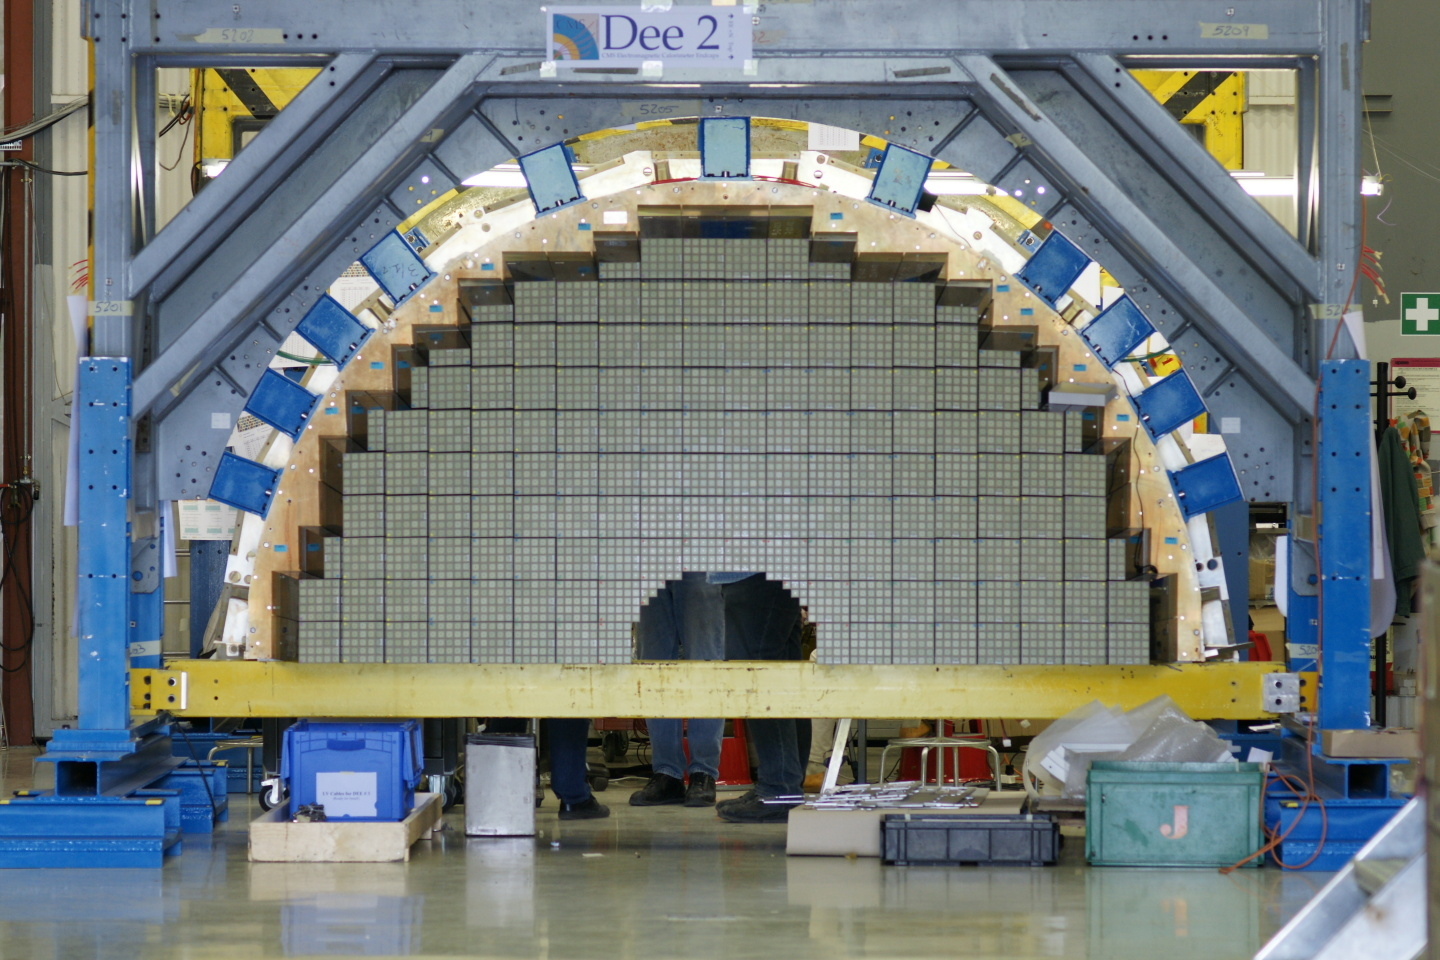
\includegraphics[width=\marginparwidth]{CMS/dee.jpg}
		\captionof{figure}{Photo d'un "Dee".}
		\label{DEE}
	}
    	\marginpar
    {
    	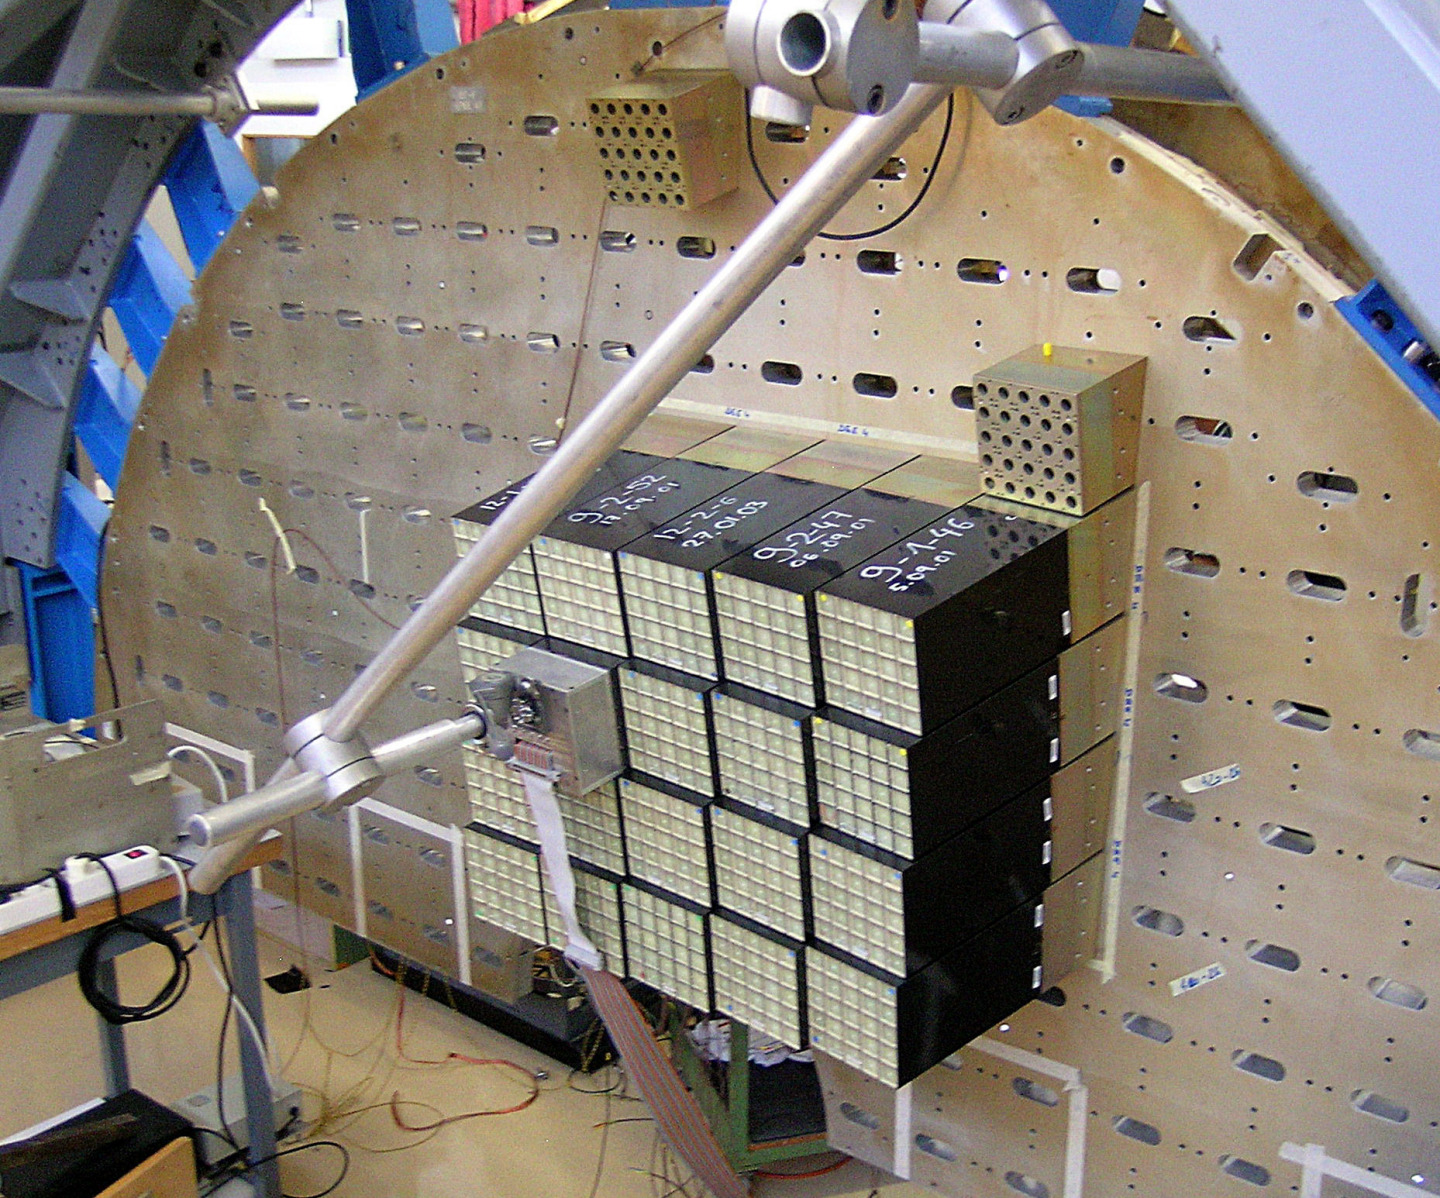
\includegraphics[width=\marginparwidth]{CMS/20SCs.jpg}
    	\captionof{figure}{Photo du montage de 20 Super-Crystaux sur un des Dee.}
    	\label{SP}
    }
  	\marginpar
{
	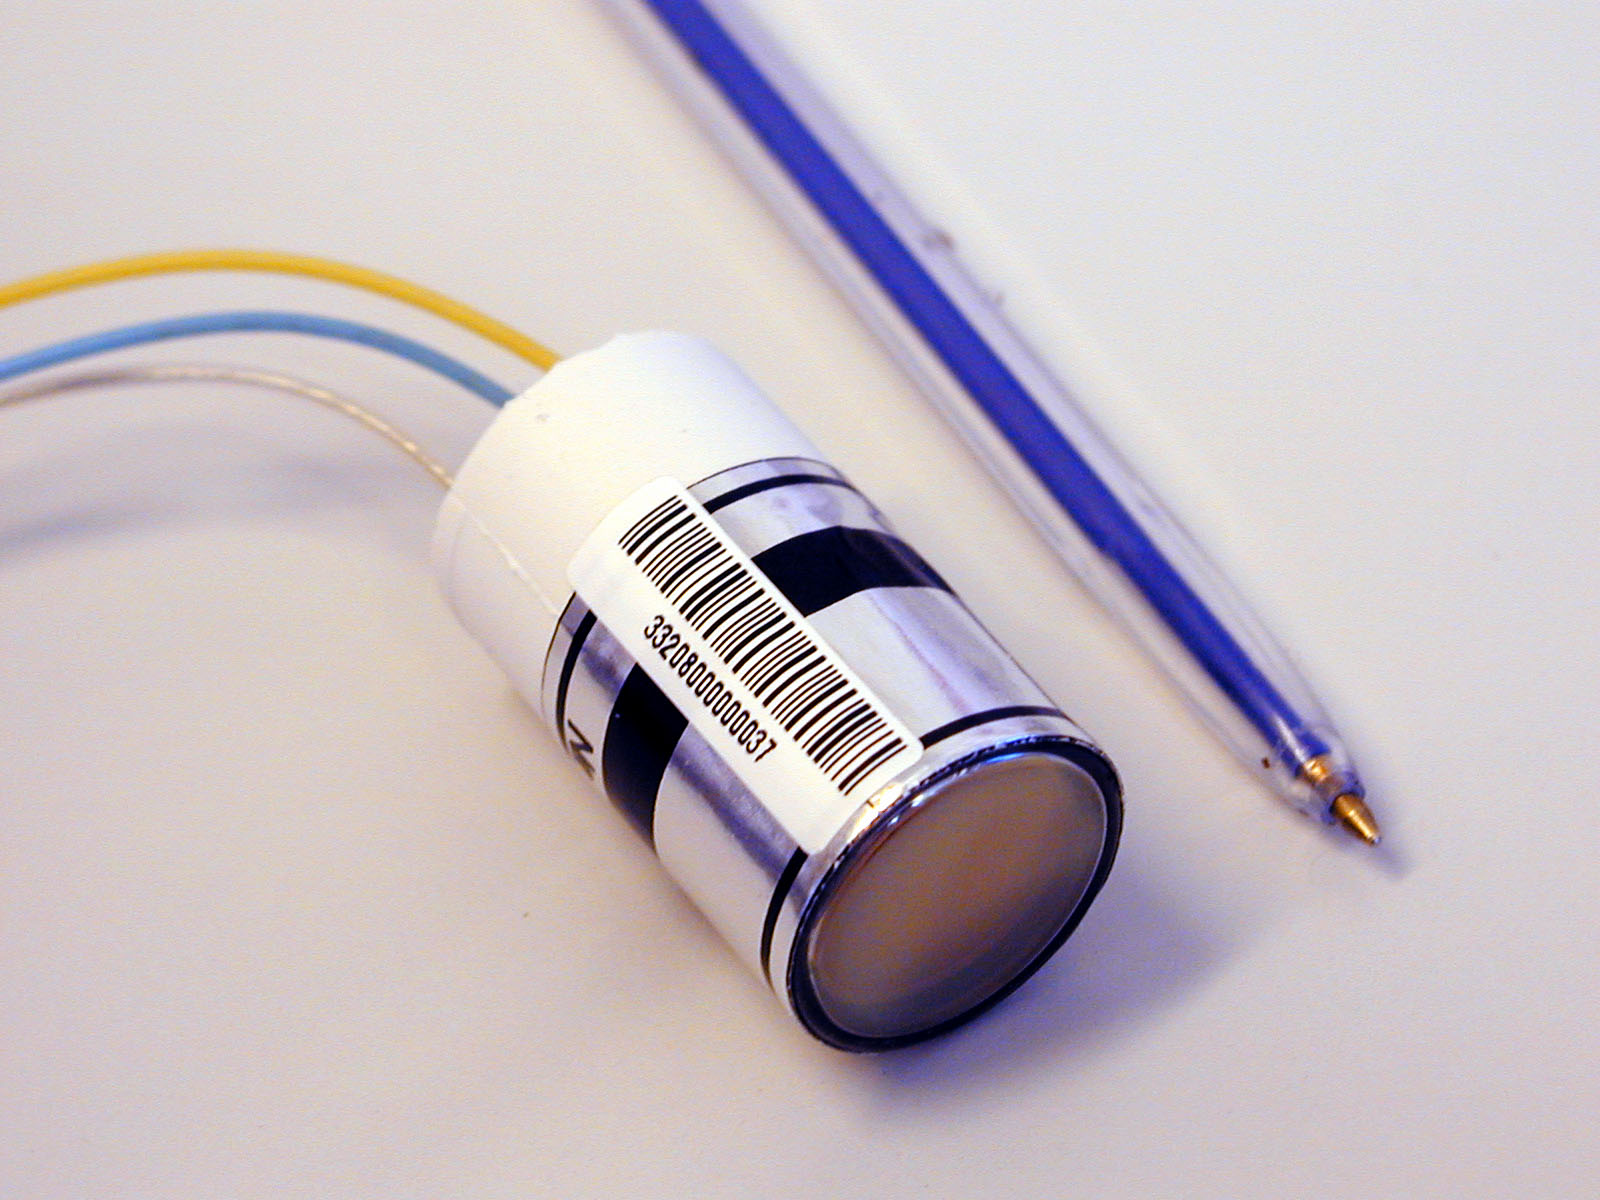
\includegraphics[width=\marginparwidth]{CMS/VPT.jpg}
	\captionof{figure}{Photo d'une VPT.}
	\label{VPT}
}

   Les crystaux de PbWO4 ont une grande densité ($\rho=$8.28g.cm$^{-3}$) une longueur d'interaction $X_{0}$ assez courte de 0.89cm est un petit rayon de molière ($r_{M}$=2.2cm) ainsi qu'une grande vitesse de radiation (80\% dans 25 ns). 
	\item \textbf{L'initiateur de gerbe } (cf.fig\ref{PRESHOWER}), appellé \textit{Preshower} est placé entre le EB et le EE. Il consiste en deux couches de détecteurs de silicium de pas 1.9mm intercalé entre deux couches en plomb (2$X_{0}$ devant et 1$X_{0}$ derrière la première couche de silicium ). Il permet d'améliorer la précision de la mesure de la position de la gerbe électromagnétique et le discrimination $\gamma \pi_{0}$. Il couvre une région comprise entre 1.653<$|\eta|$<2.6
	  \begin{figure}[ht!]
		\centering
		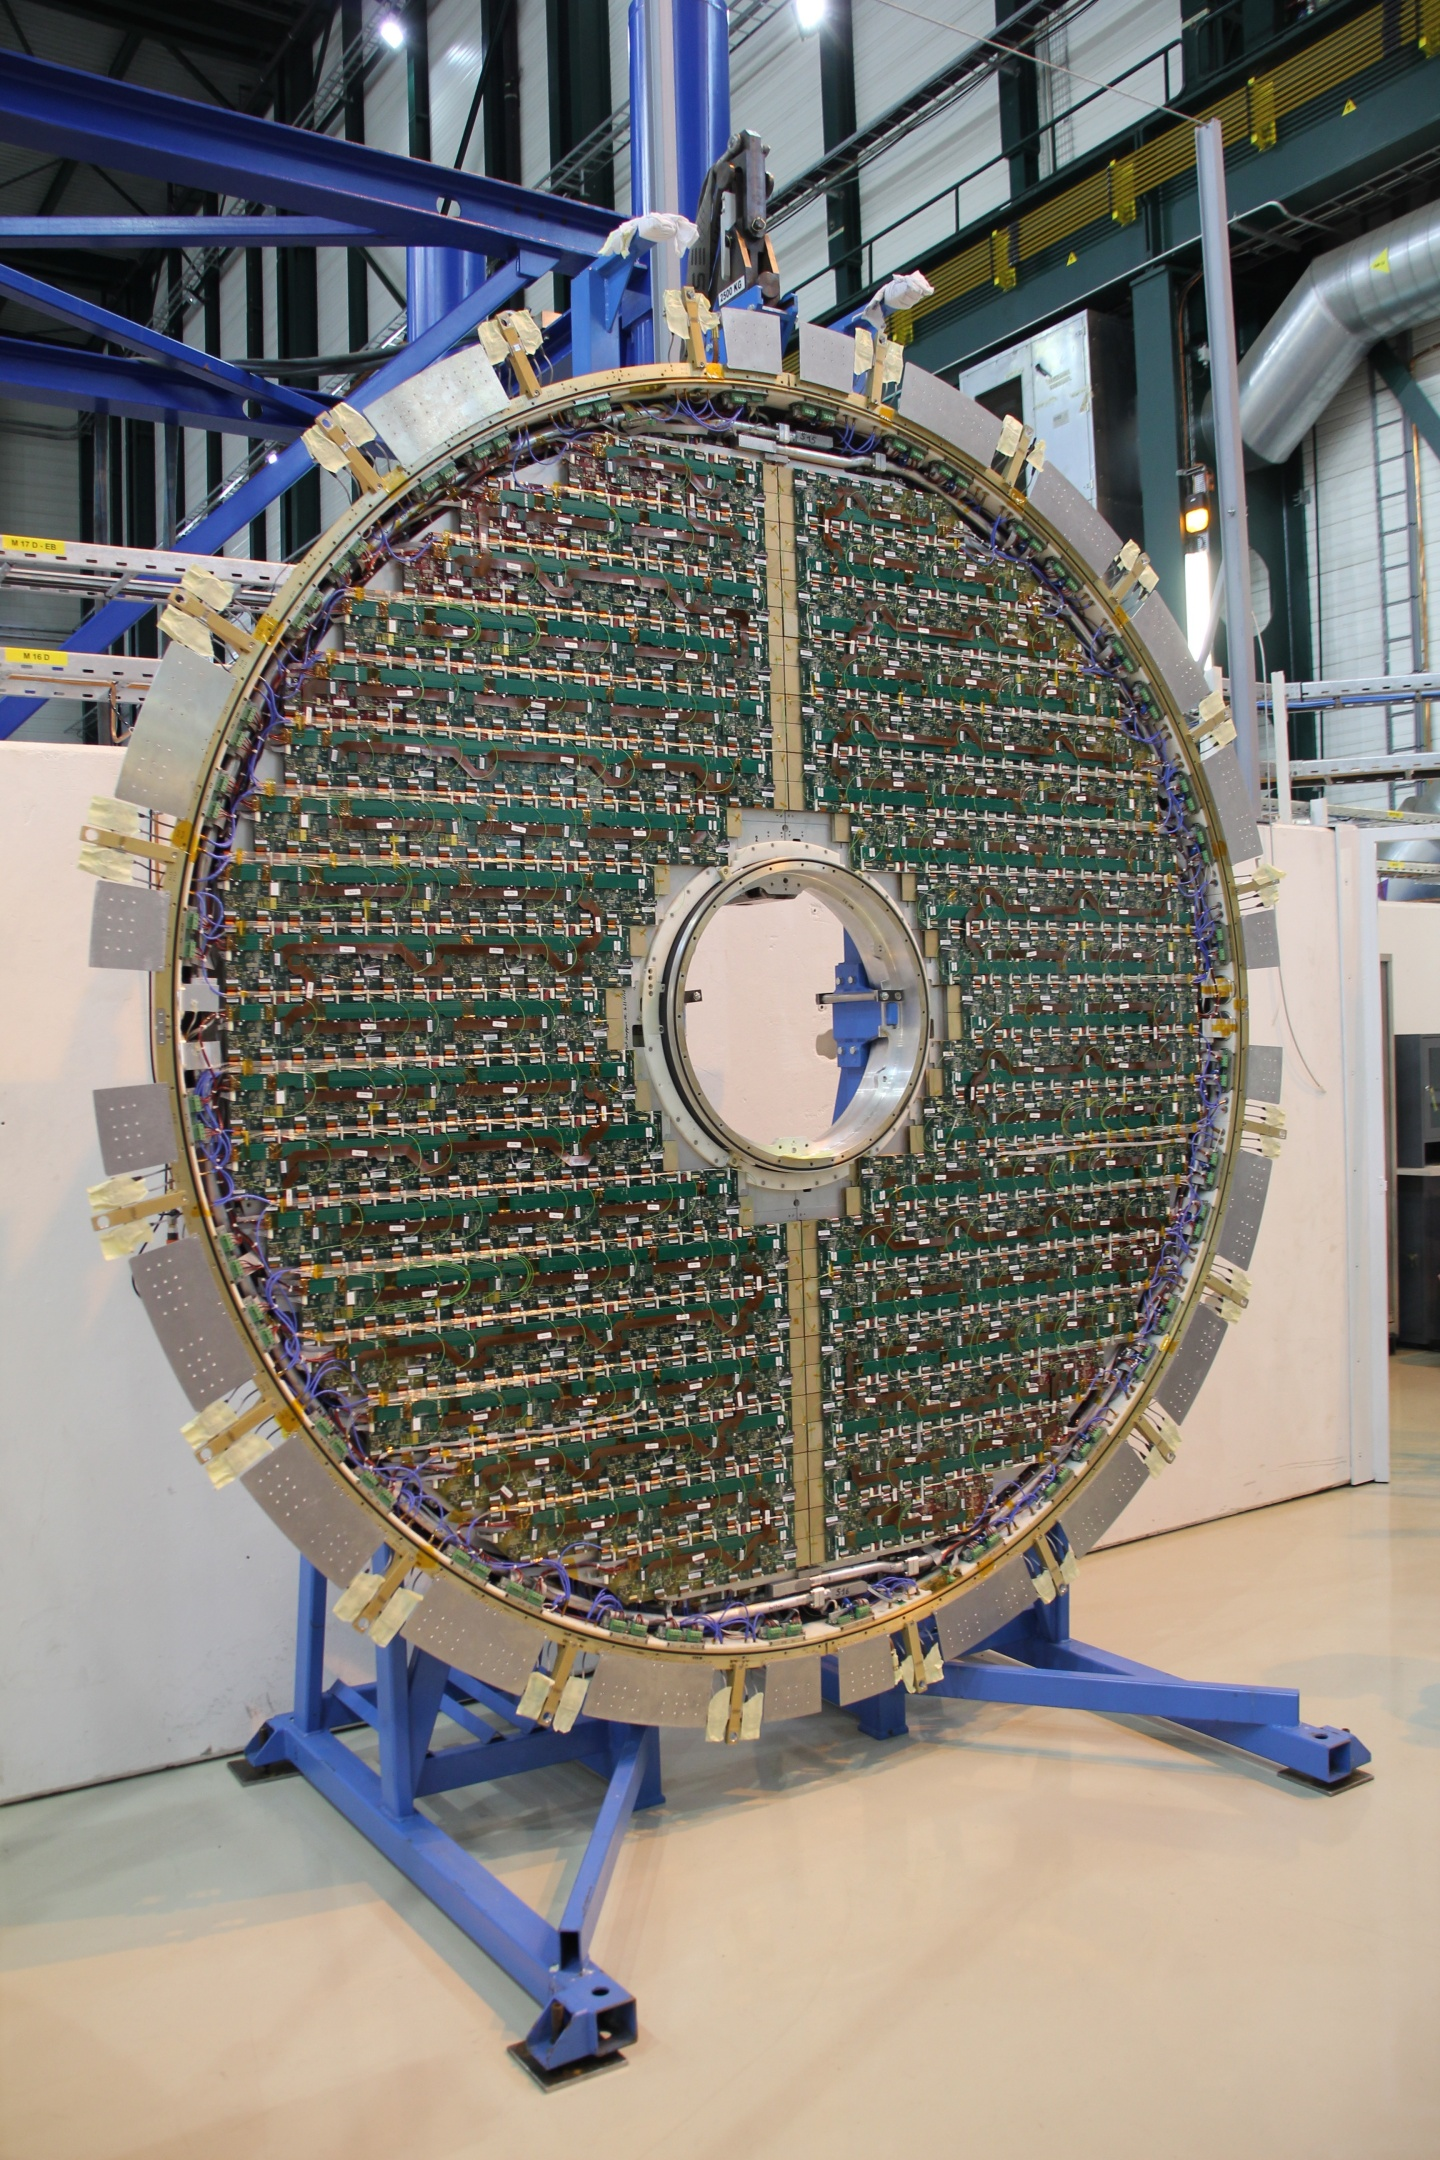
\includegraphics[width=0.3\textwidth]{CMS/preshower.jpg}
		\captionof{figure}{Photo d'un des preshower.}
		\label{PRESHOWER}
	\end{figure}
\end{itemize}
\subsection{Le calorimètre hadronique}
